\chapter{Diseño e implementación} % Main chapter title
\label{ChapterDisenoImplementacion} 


%----------------------------------------------------------------------------------------
%	SECCIÓN - HARDWARE
%----------------------------------------------------------------------------------------



\section{Hardware}
En la siguiente sección se detallan las consideraciones que se tuvieron en cuenta al momento de diseñar la arquitectura de hardware del proyecto como también los distintos componentes que se seleccionaron para su fabricación. 

\subsection{Arquitectura del sistema de nodos}
\label{sec:arquitecturahardware}

El principal desafío del proyecto fue establecer una red de comunicación entre múltiples nodos que puedan medir datos y transmitirlos a través de una red móvil hacia Internet. Los principales requerimientos que condicionaron la elección de la arquitectura y la tecnología a implementar fueron:

\begin{itemize}
    \item Acceso a Internet mediante red móvil: los nodos deben tener la capacidad de transmitir los datos a través de la red móvil debido a la necesidad de acceso a Internet en áreas extensas y remotas. 
    \item Eficiencia en costos y simplicidad: la solución debe ser sencilla y barata de implementar, especialmente en lo que refiere al hardware de los microcontroladores.
    \item Alcance y cobertura extensa: el sistema debe ser capaz de operar en áreas donde las distancias entre los nodos y el punto de acceso a Internet pueden ser de hasta 500 metros, lo que excluye tecnologías de corto alcance como el Wi-Fi.
\end{itemize}


\subsubsection{Análisis de Tecnologías de Acceso a Internet}

Se evaluaron distintas tecnologías para permitir el acceso a Internet de forma inalámbrica:

\begin{itemize}
    \item Wi-Fi: aunque es una tecnología de bajo costo y ampliamente soportada, tiene limitaciones importantes en cuanto a su alcance y capacidad de penetración en entornos remotos o con obstáculos. Por este motivo, se descarta para cubrir áreas extensas.
    \item Redes Móviles (GSM, 3G, 4G): se optó por utilizar la red móvil, ya que ofrece una solución más robusta en términos de cobertura geográfica y fiabilidad. Entre las alternativas, la tecnología 4G se destaca por ofrecer una mayor velocidad y mejor latencia, ideal para enviar los datos recolectados por los nodos sensores. 
    Dado que equipar a cada nodo con su propio módulo de acceso a red móvil implicaría un costo elevado y mayor mantenimiento, esta opción es descartada. Por lo tanto, no se dará acceso individual a cada nodo a la red móvil.
\end{itemize}



\subsubsection{Solución Propuesta: topología en Estrella}

Para resolver el problema de costos y complejidad, se optó por una topología en estrella donde sólo un nodo tiene acceso a la red móvil. Los demás nodos se comunicarán con este nodo a través de una red de radio local. Así nace la topología Nodo AP - Nodo Sensor:

\begin{itemize}
    \item Nodo AP (Access Point): se encarga de la comunicación con la red móvil. Este nodo tiene el hardware necesario para enviar los datos recolectados a través de Internet.
    \item Nodos Sensor: estos nodos estarán dispersos por el área a monitorear y se encargan de realizar las mediciones necesarias. Luego, transmiten sus datos al Nodo AP a través de una tecnología de radio.
\end{itemize}

El Nodo AP actúa como enrutador, permitiendo la recolección y posterior transmisión de los datos de los Nodos Sensores hacia Internet.

\subsubsection{Selección de la Tecnología de Comunicación entre Nodos}

Dado que los nodos deben estar dispersos en áreas extensas y la comunicación requiere bajo consumo de energía, se evaluaron las siguientes tecnologías:
\begin{itemize}
    \item Wi-Fi: aunque es una opción común, fue descartada debido a su alcance limitado y alto consumo energético.

    \item Bluetooth: ofrece bajo consumo, pero también tiene un alcance limitado y no es adecuado para transmitir datos a largas distancias.
    
    \item ESP-NOW: es eficiente en consumo energético y funciona bien con dispositivos ESP, pero presenta dos desventajas. Está limitado a la tecnología de Espressif y tiene un alcance menor en comparación con otras opciones.

    \item LoRa: es la opción ideal debido a su gran alcance y bajo consumo energético. Aunque tiene un \textit{bitrate} bajo, es suficiente para la transmisión de las mediciones necesarias, y su capacidad de penetración en ambientes rurales o con obstáculos lo convierte en la mejor opción para este proyecto.
    
\end{itemize}

\subsubsection{Definición final}

La arquitectura e implementación final seleccionada es una red en topología estrella donde:

\begin{itemize}
    \item Los Nodos AP tendrán acceso a la red móvil y actuarán como intermediarios entre los Nodos Sensores y la red de Internet.
    \item Los Nodos Sensores utilizarán LoRa para comunicarse con los Nodos AP, aprovechando su largo alcance y bajo consumo de energía.
\end{itemize}

Esta solución reduce el costo y el mantenimiento, y asegura una comunicación efectiva en áreas con distancias extensas y condiciones adversas para otras tecnologías de radio.

\subsection{Diseño de los Nodos}

En las figuras \ref{fig:DisNodoSensor} y \ref{fig:DisNodoAP} se presenta en formato de diagramas de bloques los principales componentes que conforman cada uno de los nodos del proyecto.



\begin{figure}[H]
    \centering
    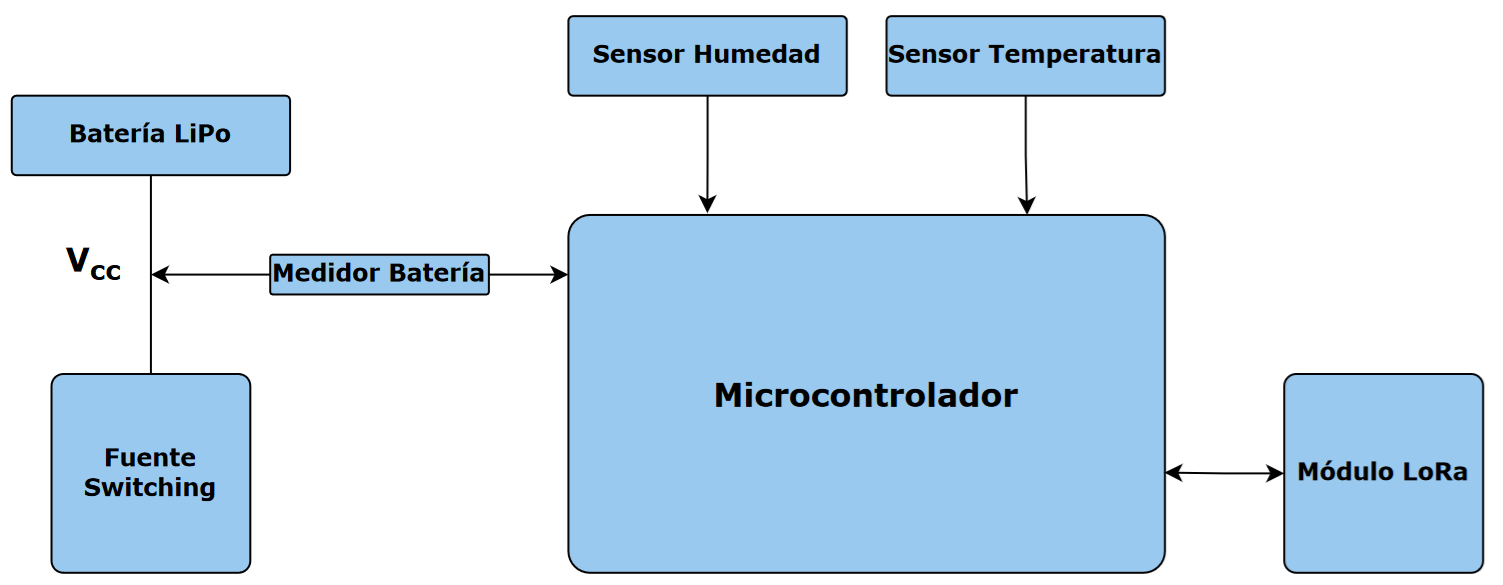
\includegraphics[width=1\linewidth]{Figures/Hardware/Modulos/nodo_sensor.png}
    \caption{ Diagrama de diseño del Nodo Sensor.}
    \label{fig:DisNodoSensor}
\end{figure}

\begin{figure}[H]
    \centering
    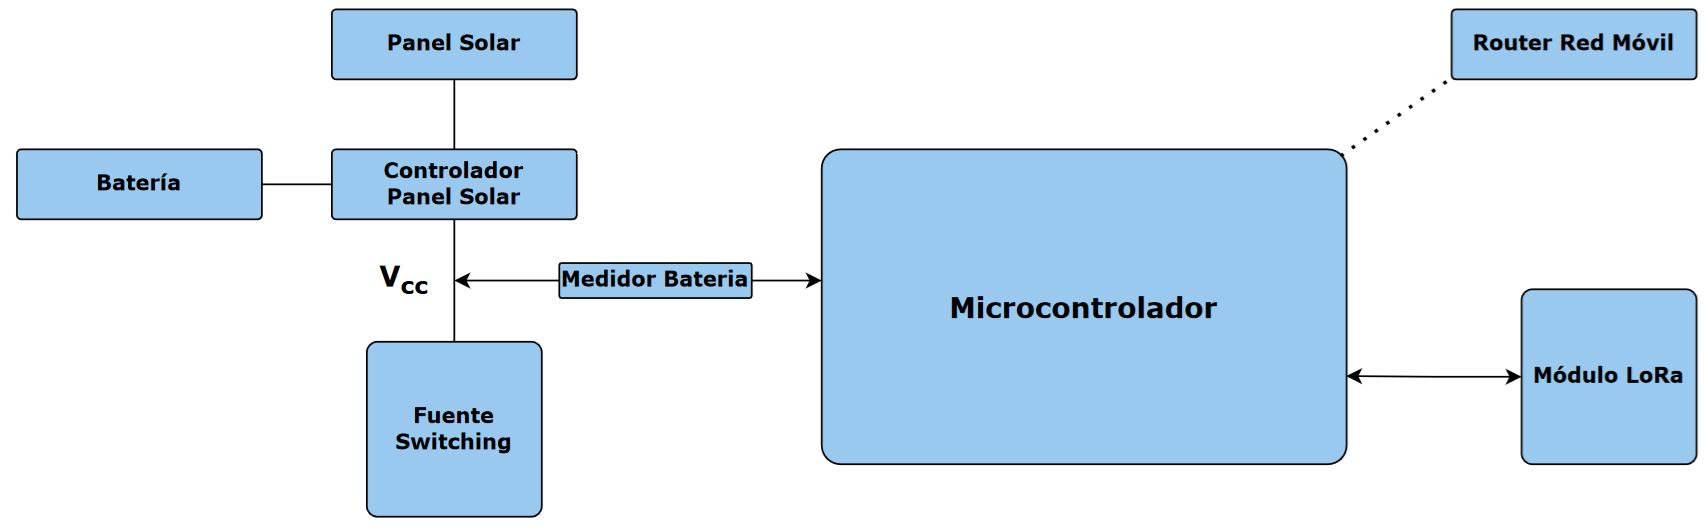
\includegraphics[width=1\linewidth]{Figures/Hardware/Modulos/nodo_ap.png}
    \caption{Diagrama de diseño del Nodo Access Point.}
    \label{fig:DisNodoAP}
\end{figure}


\subsection{Especificación técnica de los Nodos}
\label{sec:DescrModulos}

\subsubsection{Microcontrolador: ESP-WROOM-32.}

\label{sec:Microcontrolador}
\begin{figure}[H]
	\centering
	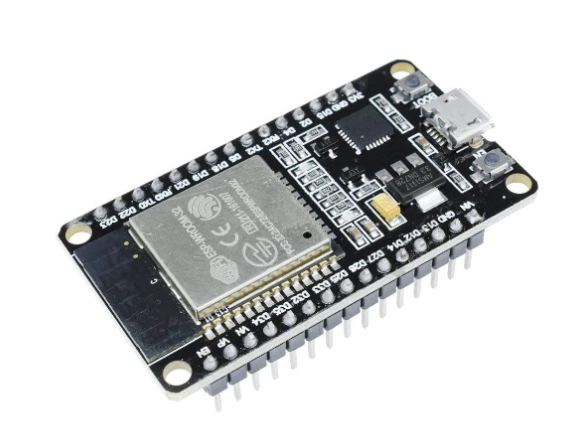
\includegraphics[scale=1]{./Figures/Hardware/Modulos/esp32.png}
	\caption{Microcontrolador ESP-WROOM-32.}
	\label{fig:Microcontrolador}
\end{figure}

El modulo microcontrolador que se utiliza en el proyecto es el ESP-WROOM-32 (ver figura \ref{fig:Microcontrolador}), módulo desarrollado por Espressif.

Características principales (véase \cite{Esp32Datasheet} y \cite{Esp32WroomDatasheet}):
\begin{itemize}
    \item Microcontrolador ESP32: el núcleo del ESP-WROOM-32 es el chip ESP32, que incluye dos núcleos de CPU capaces de funcionar a hasta 240 MHz, permitiendo manejar múltiples tareas en paralelo.
    \item Conectividad Wi-Fi: soporta los estándares IEEE 802.11 b/g/n (2.4 GHz).
    \item Memoria RAM 520 KB de SRAM.
    \item Memoria Flahs 4MB.
    \item I/O: múltiples GPIO que soportan distintas interfaces y protocolos como UART, SPI, I2C, PWM, ADC y DAC.
    \item Bajo consumo energético: cuenta con varios modos de ahorro de energía, como el modo de suspensión profunda (\textit{Deep Sleep}).
    \item Tensión de funcionamiento: 3.3 V, con la capacidad de manejar entradas externas de 5 V mediante reguladores integrados.
\end{itemize}

La elección del microcontrolador se fundamentó tanto en las prestaciones tecnológicas que ofrece, como en su precio competitivo y su disponibilidad en el mercado argentino.

\subsubsection{Capa de Enlace por Radio: LoRa SX1278}

\begin{figure}[H]
	\centering
	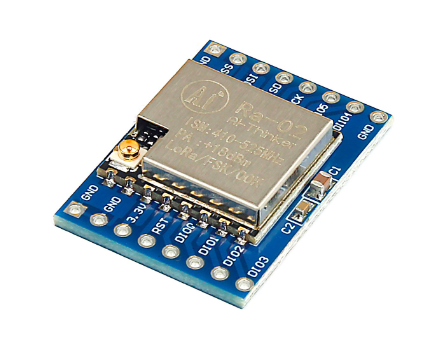
\includegraphics[scale=1]{./Figures/Hardware/Modulos/LoRa.png}
	\caption{Modulo LoRa SX1278.}
	\label{fig:LoRa}
\end{figure}

\label{sec:LoRa}
El modulo LoRa que se utiliza en el proyecto es el LoRa SX1278 (ver figura \ref{fig:LoRa}). Se trata de un transceptor de radiofrecuencia, que se caracteriza por permitir la comunicación de largo alcance con bajo consumo de energía. Este módulo es ampliamente utilizado debido a su robustez en condiciones adversas y su capacidad de operar en frecuencias no licenciadas (véase \cite{LoraDatasheet}).

Características principales:
\begin{itemize}
    \item Chip SX1278: el núcleo del módulo es el chip SX1278 de Semtech, que utiliza la modulación LoRa para ofrecer comunicación de largo alcance con una excelente sensibilidad y resistencia a las interferencias.
    \item Frecuencia de operación: 433 MHz.
    \item Alcance: el módulo puede lograr un rango de comunicación de hasta 10 km en condiciones ideales (línea de vista).
    \item Bajo consumo de energía: El SX1278 puede operar de manera eficiente en términos de consumo energético, lo que lo convierte en una excelente opción para aplicaciones alimentadas por baterías o dispositivos que requieren largos periodos de operación con poca energía. En el Sleep mode el consumo puede ser de apenas microamperios
    \item Tensión de funcionamiento: 3.3 V.
    \item Interfaz de comunicación: se comunica con el microcontrolador principal a través de la interfaz SPI (Serial Peripheral Interface)
    \item Protección y robustez: el módulo está diseñado para ser resistente a interferencias, lo que lo hace adecuado para operar en entornos con altos niveles de ruido electromagnético.
\end{itemize}

El módulo LoRa SX1278 es una solución de comunicaciones de largo alcance y bajo consumo, ideal para aplicaciones IoT donde la robustez y la eficiencia energética son clave. Su capacidad de operar en frecuencias sin licencia y su fácil integración con microcontroladores lo hacen una opción popular para proyectos de redes inalámbricas. Al igual que el microcontrolador, la selección de este módulo se basó en sus prestaciones tecnológicas anteriormente descritas y en su disponibilidad y precio en el mercado argentino.

\subsubsection{Acceso Red Móvil: SIM800L vs Router 4G}

\begin{figure}[H]
    \centering
    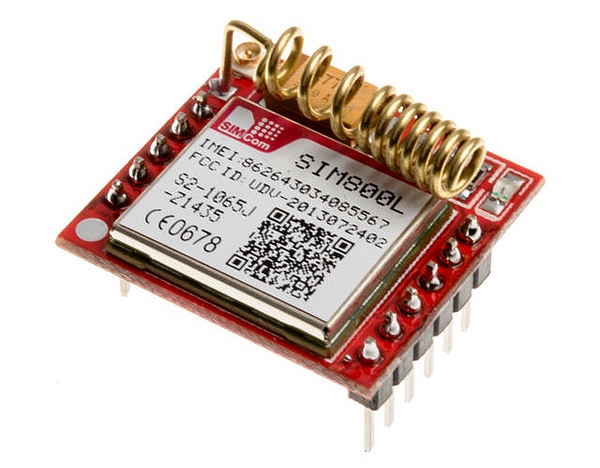
\includegraphics[width=0.5\linewidth]{Figures//Hardware//Modulos/1-SIM800L-Module.jpg}
    \caption{Módulo GSM SIM800L.}
    \label{fig:enter-label}
\end{figure}

\label{sec:capaTransporte}

En el desarrollo del proyecto, uno de los desafíos principales fue asegurar la conectividad a la red móvil para transmitir los datos recolectados por los nodos. Inicialmente, se optó por el uso del módulo SIM800L debido a su bajo costo y compatibilidad con las redes GSM.

El SIM800L es un módulo que trabaja en las bandas GSM/GPRS permitiendo la transmisión de datos por HTTP con una interfaz serie por comandos AT (véase \cite{SIM800Datasheet}).
Si bien es de bajo costo y consumo energético durante las pruebas de su implementación se presentaron varios problemas relacionados no solo con la alimentación y el consumo energético de dicho módulo, sino también con la complejidad y falta de robustez y velocidad de la comunicación

Se ha llegado inclusive a desarrollar una herramienta propia para su debido manejo, el cual consistió en un sistema Winforms para comandar el equipo y expresar todas sus capacidades (ver figura \ref{fig:aplicativoSIM800L}):

\begin{figure}[H]
    \centering
    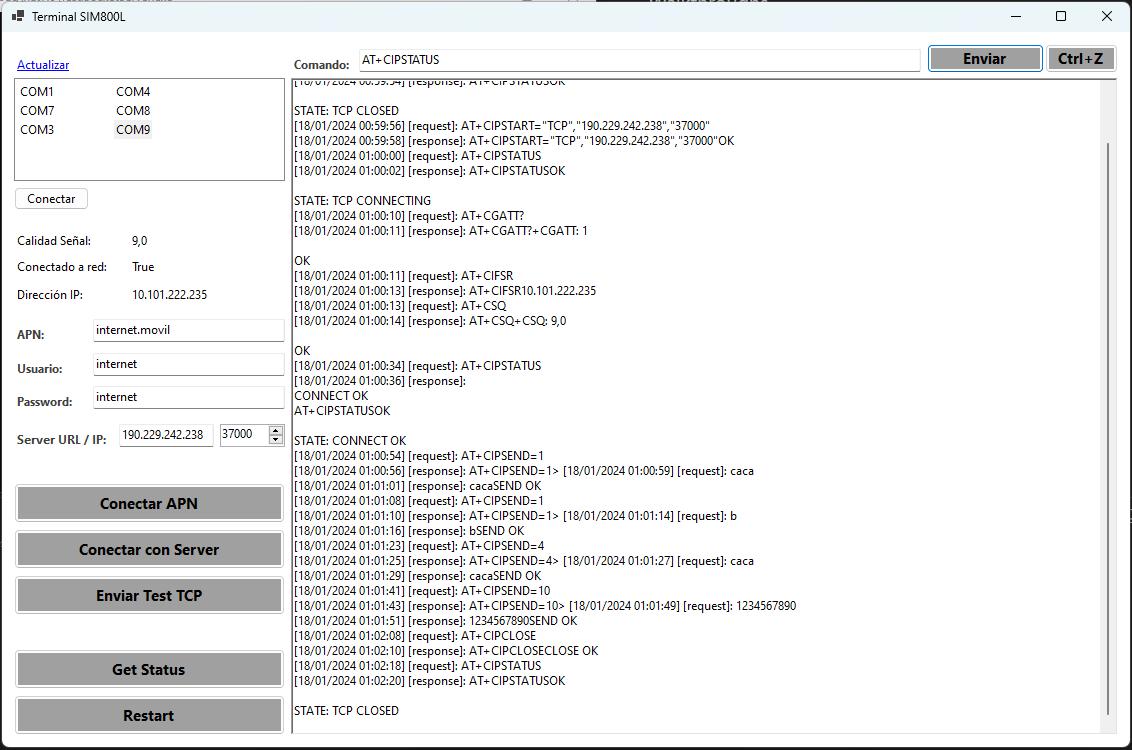
\includegraphics[width=1\linewidth]{Figures/Firmware/admin_gsm.png}
    \caption{Aplicativo de escritorio de administracion del SIM800L.}
    \label{fig:aplicativoSIM800L}
\end{figure}

El módulo SIM800L presentó los siguientes inconvenientes:

\begin{itemize}
    \item Problemas de alimentación: el SIM800L requiere una fuente de alimentación estable y capaz de proporcionar picos de corriente de hasta 2A durante su funcionamiento. En nuestra implementación, esto resultó ser problemático, ya que las fuentes de alimentación disponibles no lograban satisfacer estos picos de corriente, causando inestabilidad en la conexión.
    
    \item Altas demandas energéticas: el consumo energético del SIM800L es considerable, lo cual no es ideal para un proyecto en el que se busca optimizar el uso de energía, especialmente en aplicaciones de nodos remotos donde la disponibilidad de energía es limitada. Si bien el módulo cuenta con modos de ahorro de energía, el consumo durante su funcionamiento normal es excesivo para los requisitos del proyecto.
    
    \item Cortes de comunicación: debido a la falta de una alimentación adecuada, el módulo experimentaba desconexiones frecuentes de la red, lo que afectaba la confiabilidad del sistema en su conjunto.
\end{itemize}

Debido a estos inconvenientes, se decidió evaluar otras alternativas que ofrecieran mayor estabilidad en la alimentación y una menor complejidad de integración a nivel \textit{firmware}.

Después de los problemas enfrentados con el SIM800L, se optó por migrar a un router de red móvil USB:

\begin{figure}[H]
    \centering
    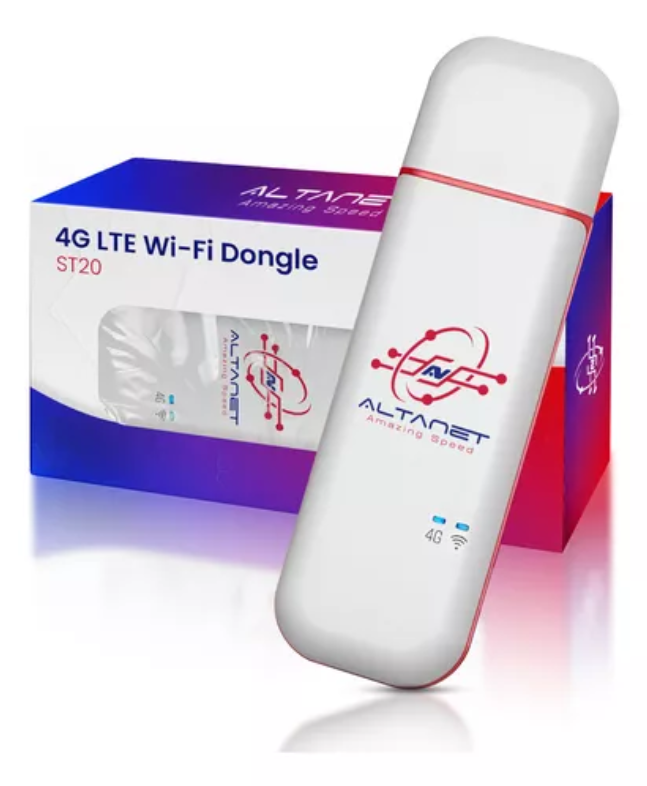
\includegraphics[width=0.6\linewidth]{Figures//Hardware//Modulos/dongle.png}
    \caption{Router 4G portátil.}
    \label{fig:enter-label}
\end{figure}

Esta solución ofreció una serie de ventajas significativas para nuestro sistema:

\begin{itemize}
    \item Simplificación de la alimentación: esta solución se alimenta via USB tipo A, lo cual al ser un estándar no requiere ningún diseño de integración.
    
    \item Menor demanda energética: en comparación con el SIM800L, los routers portátiles móviles modernos presentan una mejor eficiencia energética, lo que permitió una reducción en el consumo de energía global del sistema.
    
    \item Conectividad más robusta: la calidad de la conexión a la red móvil ha mejorado notablemente, con menos desconexiones y una mayor capacidad para mantener la transmisión de datos incluso en condiciones de señal débil. El router portátil 4G permite conectividad 4G, mientras que el módulo SIM800L opera en la red GSM.
    
    Esta solución también ofrece la ventaja de adaptabilidad: si la red GSM dejara de estar disponible, no sería un problema gracias a esta configuración. Incluso en el caso de que la red 4G fuera reemplazada por 5G, solo sería necesario sustituir el router portátil 4G por uno compatible con 5G.
    
    \item Simplicidad en la integración: debido a que es un router Wi-Fi, no hace falta implementar nada para acceder a internet, es totalmente transparente para cualquier interfaz Wi-Fi, a diferencia de comandos AT por serie.
\end{itemize}

La migración del módulo SIM800L a un router 4G portátil fue una decisión acertada que permitió superar los problemas de alimentación y alta demanda energética que inicialmente afectaban la estabilidad de los nodos. Con el router 4G portátil, se logró una conectividad más robusta y eficiente, mejorando significativamente la fiabilidad de la solución en escenarios de campo y condiciones adversas.

A su vez, el hecho de que la interfaz de comunicación con el Nodo AP es Wi-Fi, en el futuro que dejen de existir redes 4G, se podrán migrar a nuevos dispositivos de redes móviles mas modernas.


\subsubsection{Sensor de Temperatura: DS18B20}

\begin{figure}[H]
	\centering
	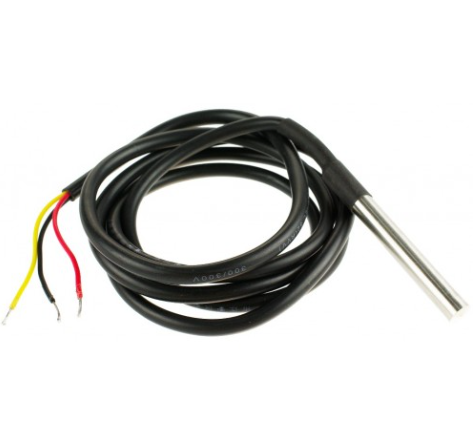
\includegraphics[scale=1]{./Figures/Hardware/Sensores/sensortemperatura.png}
	\caption{Sensor de temperatura DS18B20.}
	\label{fig:SensorTemperatura}
\end{figure}

\label{sec:SensorTemperatura}
El sensor de temperatura que se emplea en el proyecto es el DS18B20 (ver figura \ref{fig:SensorTemperatura}). Trata de un dispositivo digital  ampliamente utilizado debido a su simplicidad y precisión. A continuación se describen sus especificaciones técnicas \citep{Sensor_temp}:

\begin{itemize}
    \item Rango de temperatura: -55 °C a +125 °C.
    \item Precisión: ±0.5 °C en el rango de -10 °C a +85 °C.
    \item Resolución configurable de 9 a 12 bits.
    \item Protocolo de comunicación: 1-Wire.
    \item Tensión de operación: 5 V.
    \item Corriente de operación en modo activo aproximadamente de 1 mA
    \item Encapsulado: disponible en encapsulado TO-92 (tipo transistor) o en versiones impermeables para aplicaciones sumergidas o en exteriores.
\end{itemize}

Debido a sus excelentes prestaciones técnicas, como su amplio rango de medición, alta precisión configurable, y su capacidad para operar en entornos hostiles, el sensor de temperatura DS18B20 se presenta como una opción ideal. Además, su precio accesible, su disponibilidad y las bibliotecas bien documentadas para su implementación, hacen que sea un dispositivo ideal para este proyecto. Estas características permiten un desarrollo eficiente y confiable, sin comprometer el presupuesto ni la facilidad de integración en Argentina.

\subsubsection{Sensor de Humedad YL-69}

\begin{figure}[H]
	\centering
	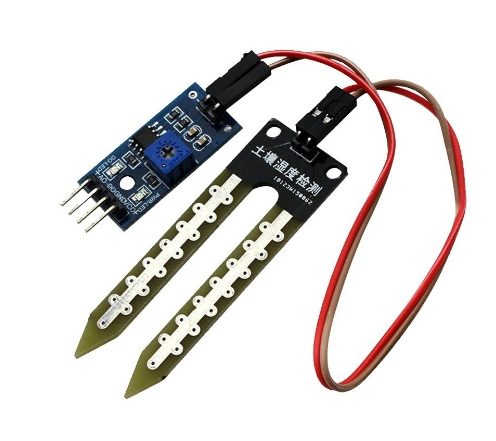
\includegraphics[scale=1]{./Figures/Hardware/Sensores/sensorhumedad.png}
	\caption{Sensor de humedad YL-69.}
	\label{fig:SensorHumedad}
\end{figure}

\label{sec:SensorHumedad}

El sensor YL-69 (figura \ref{fig:SensorHumedad}), en conjunto con el módulo controlador YL-38, permite medir el nivel de humedad en el suelo.  

Características principales:

\begin{itemize}
    \item Rango de medición: detecta niveles de humedad del suelo desde seco hasta saturado.
    \item Tensión de entrada: 3.3 V a 5 V, lo que lo hace compatible con la mayoría de plataformas de desarrollo.
    \item Salida digital (D0) y analógica (A0).
    \item Corriente de operación muy bajo.
\end{itemize}

Se trata de un sensor de humedad de suelo muy económico, lo que lo convierte en una opción asequible para proyectos de bajo presupuesto o prototipos.
Es un dispositivo relativamente fácil de conseguir en el mercado argentino.
Su estructura simple y la versatilidad que presenta al aportar salidas digitales y analógicas lo hacen un elemento adecuado para proyectos de riego y/o monitoreo.

\subsubsection{Alimentación Nodo Sensor}

\begin{figure}[H]
	\centering
	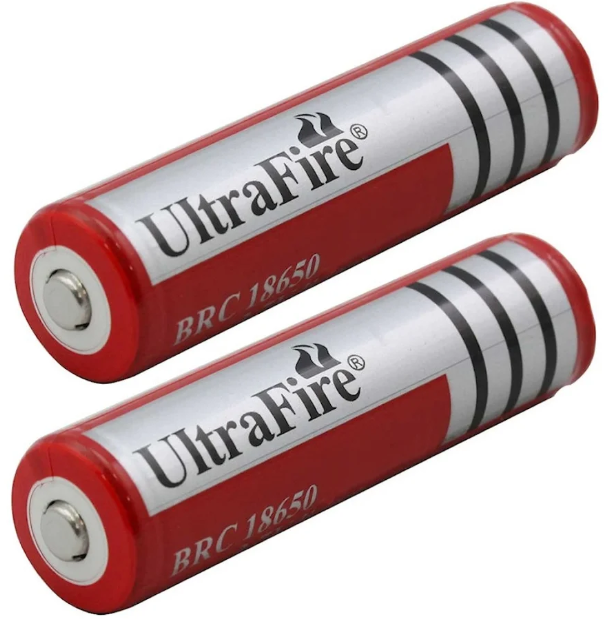
\includegraphics[scale=0.6]{./Figures/Hardware/Alimentacion/pilas.png}
	\caption{Pilas 18650.}
	\label{fig:pilas}
\end{figure}

\label{sec:AlimentacionNodoSensor}

Los Nodos Sensores utilizan dos baterías tipo 18650 conectadas en serie para proporcionar la energía necesaria. Las especificaciones de las baterías son las siguientes \cite{18650}:

\begin{itemize}
    \item Tipo de batería: 18650 de iones de litio.
    \item Capacidad nominal: entre  3500 mAh.
    \item Tensión nominal: 3.7 V por batería. Al estar conectadas en serie, el Nodo Sensor opera con una tensión combinado de 7.4V (con picos que pueden llegar hasta 8.4 V cuando las baterías están completamente cargadas).
\end{itemize}

Inicialmente, se optó por baterías de litio de 600 mAh con cargador USB debido a su tamaño compacto y facilidad de recarga. Sin embargo, en la práctica, estas baterías demostraron ser insuficientes para soportar la demanda energética de los módulos LoRa, especialmente durante los picos de consumo generados durante la transmisión de datos.

Aunque su diseño compacto y fácil integración eran ventajas, las baterías de 600 mAh no lograron proporcionar la energía necesaria, lo que resultó en fallas recurrentes y reinicios del Nodo Sensor durante las transmisiones.

Estos inconvenientes nos llevaron a replantear la fuente de energía, optando por las pilas 18650 como alternativa. Estas ofrecen una solución mucho más eficiente y confiable para alimentar los módulos LoRa, superando las limitaciones de las baterías anteriores. 

Las pilas 18650 ofrecieron varias ventajas:

\begin{itemize}
    \item Mayor capacidad energética: con una capacidad mucho mayor que las baterías de litio de 600 mAh, las pilas 18650 proporcionaron suficiente energía para alimentar los LoRa de manera continua, incluso durante los picos de demanda en la transmisión de datos.
    
    \item Estabilidad energética: las pilas 18650 proporcionan una salida de energía más estable, lo que permitió que los módulos LoRa operaran de manera más confiable, sin cortes ni reinicios inesperados.
    
    \item Duración prolongada: la mayor capacidad de las pilas 18650 extendió la duración de los nodos entre recargas, lo que redujo significativamente la necesidad de mantenimiento, especialmente en entornos remotos.
\end{itemize}

\begin{figure}[H]
	\centering
	\includegraphics[scale=0.6]{./Figures/Hardware/Alimentacion/mini360.png}
	\caption{Regulador Mini-360.}
	\label{fig:mini360}
\end{figure}

Para adaptar la alimentación a los requerimientos del proyecto se utiliza un regulador de tensión Mini-360\cite{MINI360}. Este es un regulador \textit{buck} de alta eficiencia que permite reducir la tensión de entrada de las baterías a un nivel adecuado (5 V) para los nodos. Sus especificaciones principales son las siguientes:

\begin{itemize}
    \item Tensión de entrada: 4.75 V a 23 V.
    \item Tensión de salida: regulable, ajustado a 5 V.
    \item Corriente de salida: hasta 1.8 A.
\end{itemize}

Para realizar el seguimiento del estado de carga de las baterías, se implementó un divisor resistivo que se muestra en la figura \ref{fig:DivresistivoBat}.

\begin{figure}[H]
	\centering
	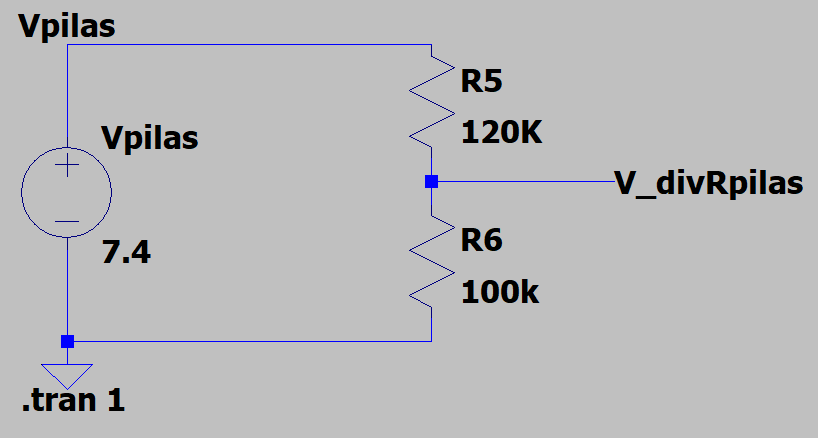
\includegraphics[scale=0.6]{./Figures/Hardware/Alimentacion/divisor_pilas.png}
	\caption{Divisor resistivo batería.}
	\label{fig:DivresistivoBat}
\end{figure}

El divisor resistivo está configurado para reducir el voltaje de entrada de las baterías a un nivel seguro que puede ser leído por el microcontrolador del nodo. 
Es decir, a la salida del divisor resistivo se obtienen 3.3 V cuando las baterías estan completamente cargadas y se considera que las baterías se encuentran descargadas cuando su tensión entre bornes es de 5.6 V.

% \begin{figure}[H]
% 	\centering
% 	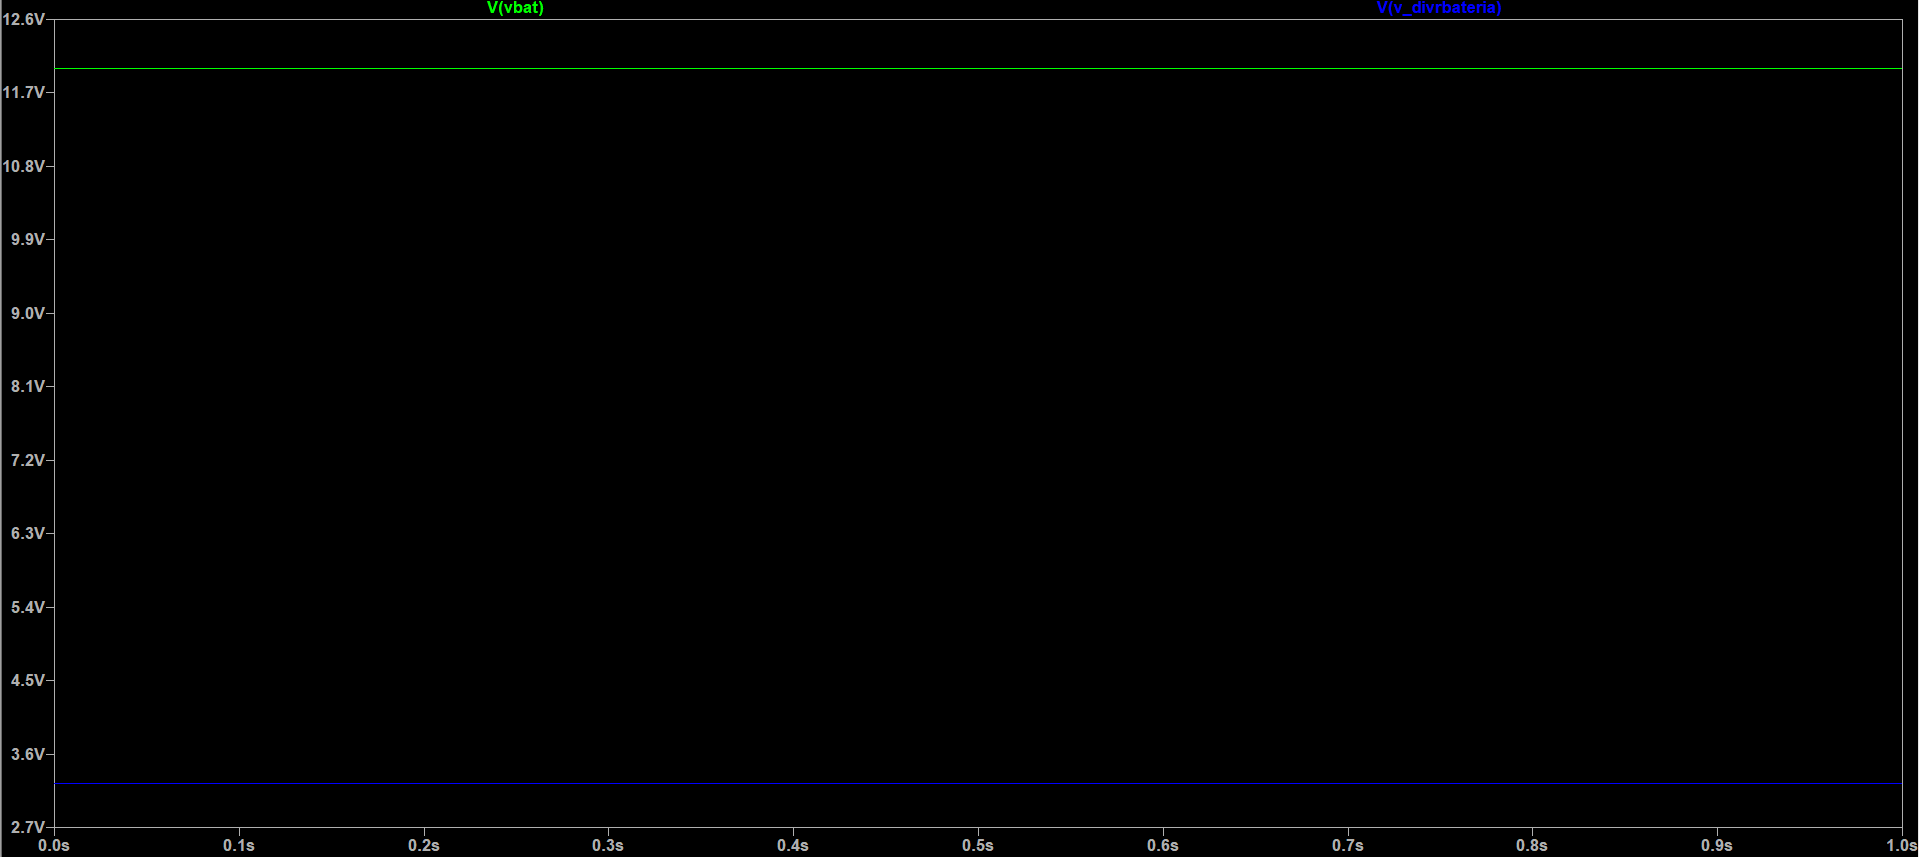
\includegraphics[scale=0.4]{./Figures/Hardware/Alimentacion/grafico_divisor_bateria.png}
% 	\caption{Grafico divisor resistivo batería}
% 	\label{fig:GrafidivresistivoBat}
% \end{figure}

\subsubsection{Alimentación Nodo AP}

\begin{figure}[H]
	\centering
	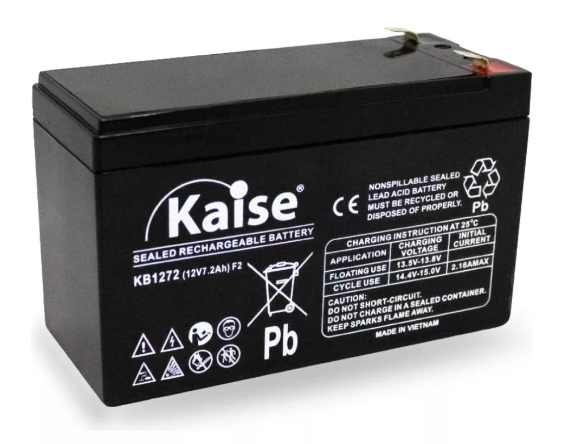
\includegraphics[scale=0.6]{./Figures/Hardware/Alimentacion/bateria.png}
	\caption{Bateria Kaise 1270.}
	\label{fig:bateria}
\end{figure}

\label{sec:AlimentacionNodoAP}

Para el Nodo Access Point, se utiliza una batería más grande para soportar mayores demandas de energía. Este nodo está alimentado por una batería de 12 V y 7 Ah marca Kaise\cite{kaise}. 
Las especificaciones de esta batería son las siguientes:

\begin{itemize}
    \item Batería Gel.
    \item Tensión nominal: 12 V.
    \item Capacidad nominal: 7 Ah.
\end{itemize}

Para mantener esta batería cargada, se emplea un panel solar de 12 V y 10 W de la marca Solar Line, que incluye un regulador  para asegurar una carga adecuada y evitar la sobrecarga o descarga profunda de la batería. El panel solar y su sistema de carga tienen las siguientes especificaciones \citep{SolarLine}:

\begin{itemize}
    \item Modelo del panel solar: Panel Solar Cargador Batería 12 V 10 WP.
    \item Potencia nominal: 10 W.
    \item Voltaje de salida: 12 V.
    \item Corriente de salida máxima del panel: aproximadamente 0.83 A.
    \item Corriente de salida máxima del regulador: aproximadamente 10 A.
    \item Salida USB: 5 V/2 A.
\end{itemize}

\begin{figure}[H]
	\centering
	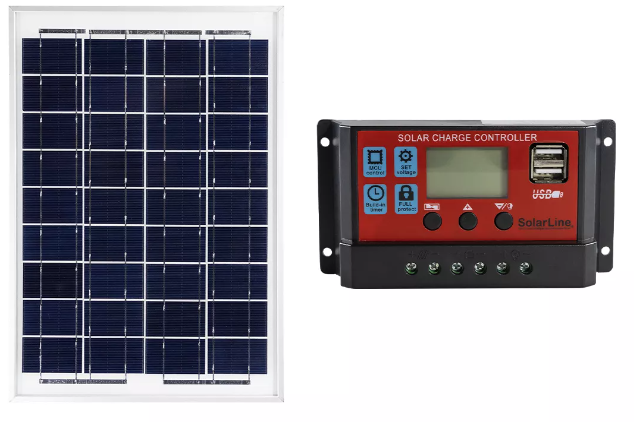
\includegraphics[scale=0.8]{./Figures/Hardware/Alimentacion/panel.png}
	\caption{Panel Solar.}
	\label{fig:panel}
\end{figure}

Al igual que el Nodo Sensor, se implementa un sistema de monitoreo del estado de las baterías mediante un divisor resistivo (ver figura \ref{fig:DivresistivoBat}).

\begin{figure}[H]
	\centering
	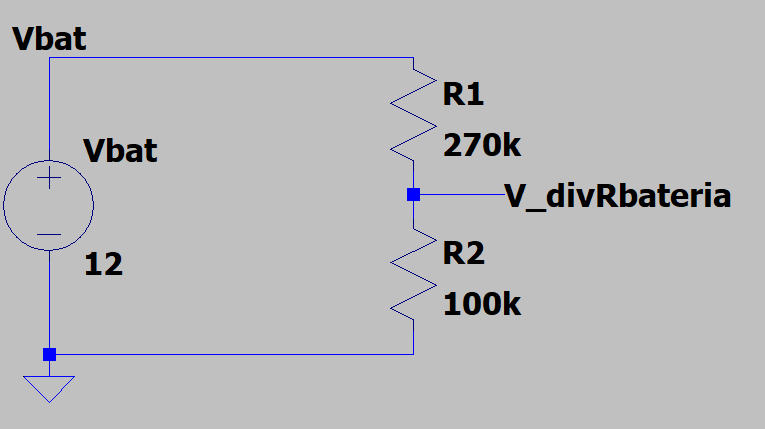
\includegraphics[scale=0.6]{./Figures/Hardware/Alimentacion/divisor_bateria.png}
	\caption{Divisor resistivo baterías.}
	\label{fig:DivresistivoBat}
\end{figure}

En este caso la tensión se reduce de 12 V a 3.3 V. Se considera que la batería se encuentra completamente cargada cuando su tensión es 12 V o más, y descargada cuando está en 9.8 V \cite{kaise}. 

%\begin{figure}[H]
%	\centering
%	\includegraphics[scale=0.4]%{./Figures/Hardware/Alimentacion/grafico_divisor_pilas.png}
%	\caption{Gráfico divisor resistivo pilas}
%	\label{fig:Grafidivresistivopilas}
%\end{figure}

\subsection{Implementación en PCB}
\label{sec:PCB}

En este trabajo se diseñaron los PCBs de los dos nodos. Dada las similitudes entre ambos se optó por diseñar un solo PCB que se adapta a ambos nodos teniendo en cuenta las siguientes diferencias:
\begin{itemize}
    \item Dependiendo del tipo de Nodo que se trate, el valor de la resistencia R1 varía. Siendo de 120 kOhm para el Nodo Sensor y 270 kOhm para el Nodo Access Point.
Esta variación se debe a la fuente de alimentación de cada Nodo (ver sección \ref{sec:AlimentacionNodoAP}).
\item En cuanto a los conectores para los sensores, las conexiones no se utilizan en el caso del Nodo Access Point.
\item Por último, tanto el microcontrolador, módulo LoRa y el regulador de tensión son comunes para los PCB de ambos Nodos Sensor y Access Point.
\end{itemize}

En la figura \ref{fig:esquematico} se nota el esquemático electrónico del proyecto.
\label{sec:EsquematicoGral}
\begin{figure}[H]
	\centering
	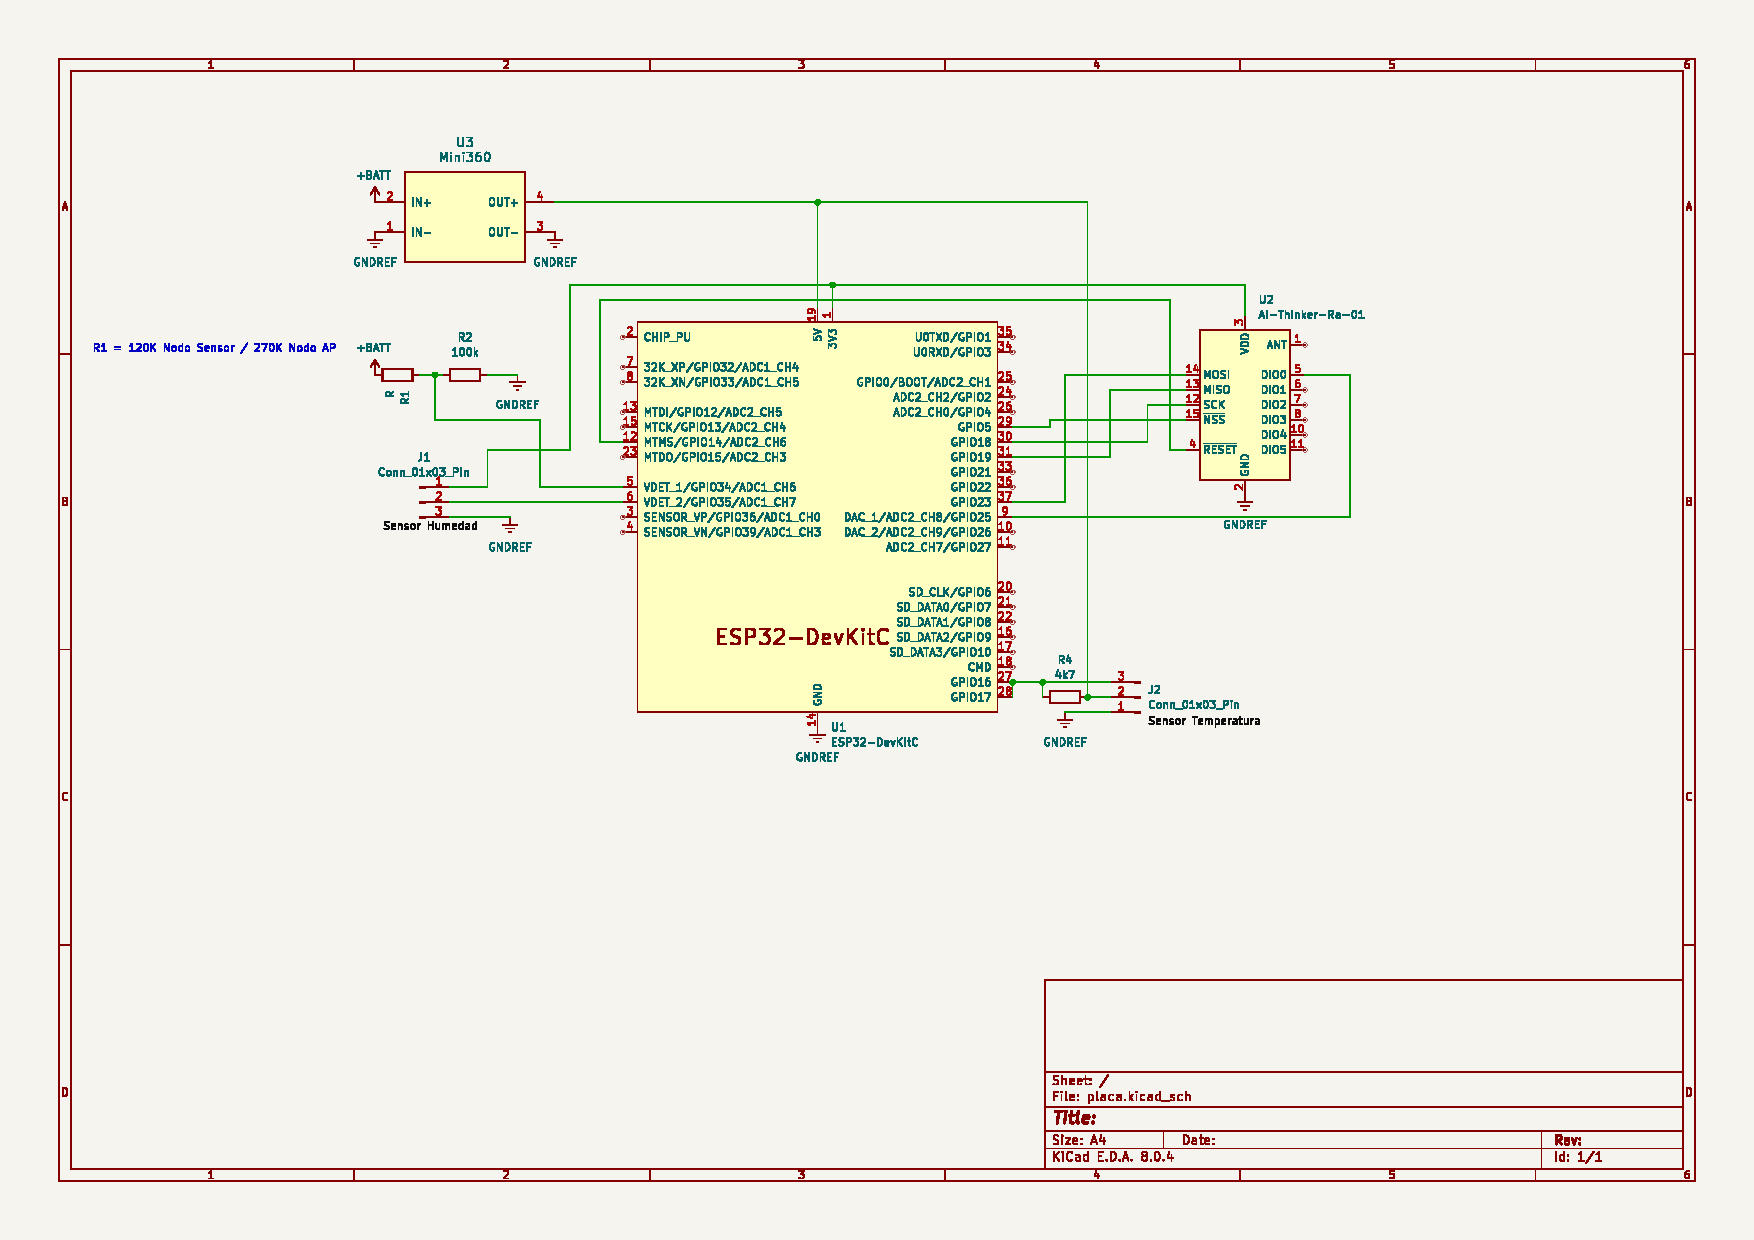
\includegraphics[scale=0.5]{./Figures/Esquematicos/esquematico.png}
	\caption{Esquemático común de los Nodos.}
	\label{fig:esquematico}
\end{figure}



Para el desarrollo del PCB se utilizó la herramienta KiCAD\citep{KiCadWebsite}. Se diseñó una placa de simple faz, sin componentes SMD, lo que facilitó su fabricación. El proceso de manufactura estuvo a cargo del Laboratorio de Circuitos Impresos (LCI) de la Facultad de Ingeniería de la Universidad de Buenos Aires.
Se aprovecha esta sección específica del PCB para agradecer al LCI por sus prestaciones y servicios y destacar la importancia de contar con un laboratorio de estas características para el desarrollo de proyectos universitarios.

En la figura \ref{fig:pcb} se muestra el PCB de los nodos.

\begin{figure}[H]
	\centering
	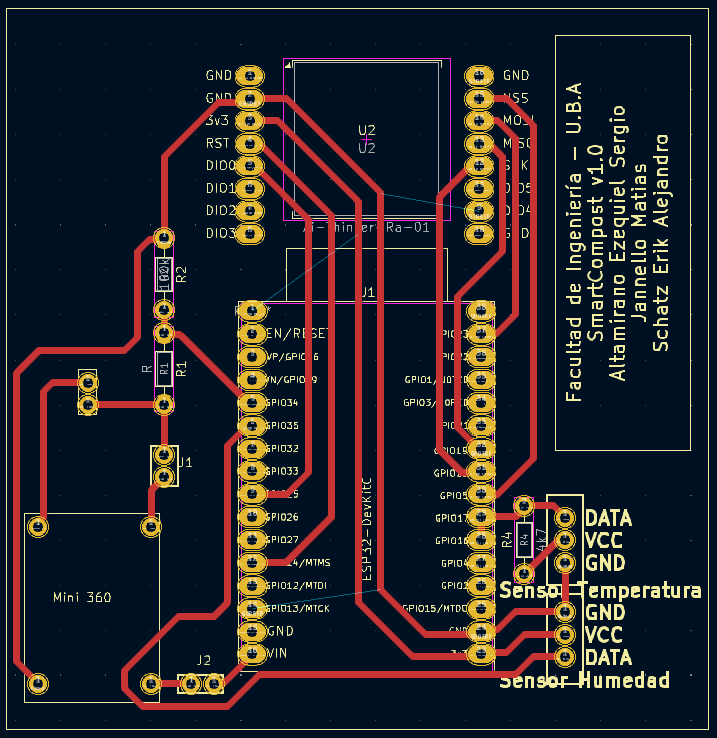
\includegraphics[scale=0.8]{./Figures/Hardware/PCB/pcb.png}
	\caption{PCB de los nodos.}
	\label{fig:pcb}
\end{figure}



Se emplearon tiras de pines hembra para montar los módulos del microcontrolador y del LoRa, conectores Molex (de 2 y 3 pines) para la conexión de los sensores y la entrada de alimentación.

También se emplearon unas tiras de pines macho (J1 y J2) para conectar jumpers. Tanto los resistores, y el regulador de tensión se soldaron directamente al PCB.
En la imagen \ref{fig:pcbFinal} se muestra el PCB en su versión con los componentes montados.

\begin{figure}[H]
	\centering
	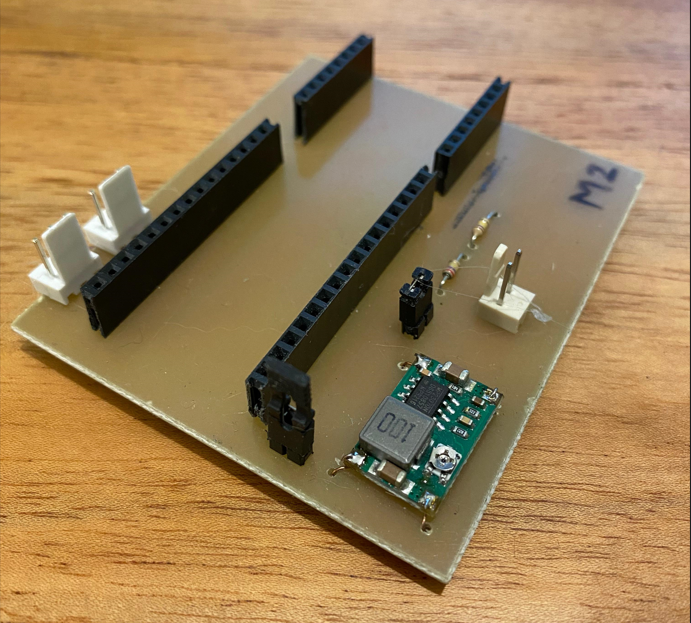
\includegraphics[scale=.8]{./Figures/Hardware/PCB/placa-final.png}
	\caption{Versión final del PCB con los componentes montados.}
	\label{fig:pcbFinal}
\end{figure}


% Agregar las demas subsecciones...

%----------------------------------------------------------------------------------------
%	SECCIÓN - FIRMWARE
%----------------------------------------------------------------------------------------

\section{Firmware}

\subsection{Arquitectura}

El firmware de SmartCompost se desarrollo en C\# utilizando  nanoFramework, una implementación optimizada para microcontroladores de 32 bits como el ESP32. Este framework permite ejecutar código administrado  facilitando el desarrollo y mantenimiento de aplicaciones embebidas.

La arquitectura del firmware está organizada en capas, lo cual garantiza una separación clara de responsabilidades y una estructura modular. En la base, el hardware y las capas de abstracción (\textit{Hardware Abstraction Layer - HAL} y \textit{Platform Abstraction Layer - PAL}) proporcionan acceso directo a los recursos del ESP32, como la CPU, la memoria, y los periféricos. Sobre estas capas, el \textit{Common Language Runtime (CLR)} gestiona la ejecución de código en un entorno seguro, proporcionando servicios como la recolección de basura, la gestión de excepciones, y funciones integradas.

Por encima de la CLR, se encuentran las bibliotecas del firmware, que incluyen módulos para la red, el manejo de hardware, e integración con servicios .NET, entre otros. Finalmente, en la capa superior, se ubican las aplicaciones de usuario y bibliotecas personalizadas, diseñadas específicamente para la lógica de negocio de SmartCompost, permitiendo la implementación de los distintos nodos y así compartiendo una lógica y diseño en común.

Esta arquitectura modular permite una implementación flexible y escalable, donde cada nodo se puede modelar según las necesidades específicas.

\begin{figure}[H]
    \centering
    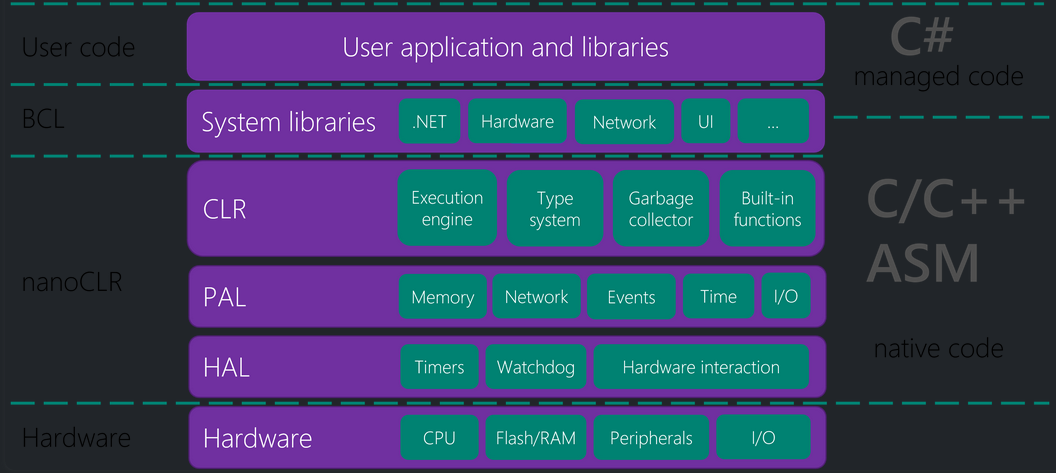
\includegraphics[width=1\linewidth]{Figures/Firmware/nanoframework_arq.png}
    \caption{Diagrama de la arquitectura del firmware.}
    \label{fig:enter-label}
\end{figure}

\subsubsection{Diseño Nodo Sensor}


El Nodo Sensor tiene como único propósito realizar las mediciones de humedad, temperatura y nivel de batería, y enviarlas hacia el Nodo Access Point. Luego debe ejecutar la rutina de \textit{DeepSleep} del ESP32 para maximizar la autonomía del mismo.

En este modo, la mayoría de los periféricos y componentes, como la CPU y la memoria flash, se apagan. Sin embargo, una pequeña parte de la RAM RTC se mantiene activa para almacenar los datos necesarios para realizar un re inicio del proyecto.

En este caso, el ESP32 está configurado para salir del DeepSleep mediante un temporizador de aproximadamente una hora. 

En la Figura \ref{fig:diagrama-flujo-sensor} se diagrama el flujo del Nodo Sensor, el cual consiste en los siguientes pasos:

\begin{figure}[H]
    \centering
    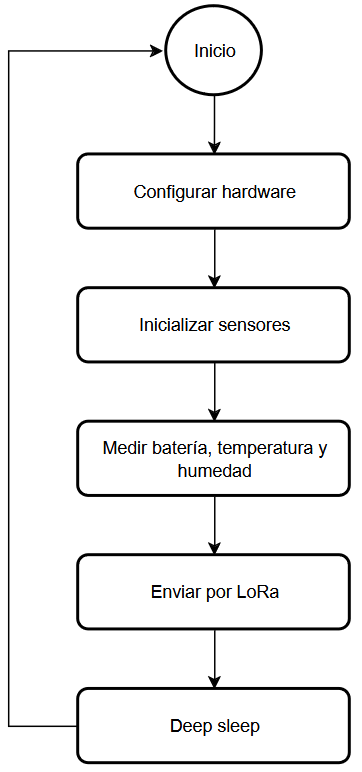
\includegraphics[width=0.5\linewidth]{Figures/Firmware/flujo_medidor.png}
    \caption{Diagrama de flujo del Nodo Sensor.}
    \label{fig:diagrama-flujo-sensor}
\end{figure}

\begin{enumerate}
    \item Configurar el hardware: aquí se configuran los respectivos pines del ESP32 para las distintas funcionalidades requeridas por los periféricos, como así también la configuración del kernel con la inicialización de los objetos requeridos para los distintos servicios utilizados (servicio Lora, servicio de logging, etc).
    \item Inicializar los sensores: se instancias los objetos para los sensores de temperatura, humedad y batería, con su debida validación para confirmar su correcto funcionamiento.
    \item Medir batería, temperatura y humedad: Para la medición de la batería y humedad, se utilizan 2 pines asociados a dos ADC distintos, y con su correspondiente transformación matemática se obtiene la magnitud deseada. En el caso del sensado de temperatura, la comunicación con el sensor DS18B20 se realiza a través del protocolo 1-Wire.
    \item Enviar por LoRa: se serializan las mediciones en un payload binario y se escriben en un bus de datos correspondientes a un módulo SPI del ESP32. El total funcionamiento del módulo LoRa SX1278 consiste en la escritura y lectura de registros del módulo a través del protocolo SPI (\cite{LoraDatasheet}).
    \item Deep sleep: una vez finalizado el envío del payload, el ESP32 es configurado para entrar en su modo Deep Sleep, el cual como indica su datasheet (\cite{Esp32Datasheet}) se deshabilitan muchas funcionalidades  que permiten un consumo total de aproximadamente $6.5 \mu A$, aumentando al máximo la autonomía del microcontrolador.
    Por otro lado, el módulo LoRa SX1278 también posee la capacidad de entrar en modo DeepSleep, el cual apaga todos los PLLs y deja sólo prendido la memoria de registros y el módulo SPI (2.1.4. Operating Modes in FSK/OOK Mode \cite{LoraDatasheet}).
\end{enumerate}

Este flujo se repite indefinidamente hasta que el Nodo se quede sin batería o se apague manualmente.

\subsubsection{Diseño Nodo Access Point}

Este Nodo tiene que como requerimiento principal en su diseño servir de punto de acceso entre los Nodos Sensor y el servicio en la nube. Por lo que debe poder actuar no sólo como enrutador, sino como \textit{buffer} de los mensajes que llegan.

En la Figura \ref{fig:diagrama-flujo-ap} se diagrama el flujo del Nodo AP, el cual consiste en una etapa de configuración y luego en la ejecución de dos hilos paralelos, junto con un hilo manejado por eventos:

\begin{figure}[H]
    \centering
    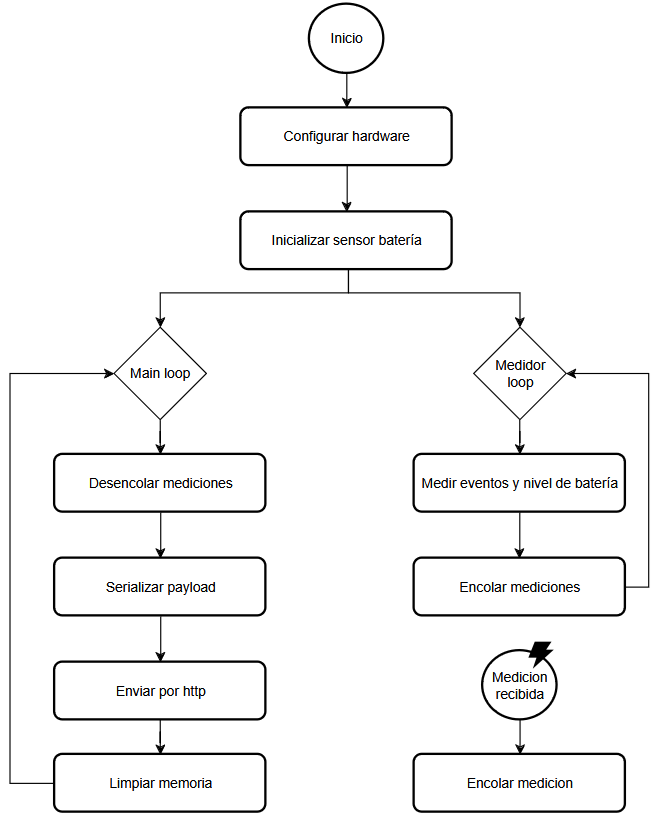
\includegraphics[width=1\linewidth]{Figures/Firmware/flujo_ap.png}
    \caption{Diagrama de flujo del Nodo AP.}
    \label{fig:diagrama-flujo-ap}
\end{figure}

La etapa de configuración consiste en la inicialización del mismo kernel descrito en el Nodo Sensor previamente, con el agregado de la configuración a la red Wi-Fi 802.11g provista por el Router 4G portátil.
El Nodo AP está provisto de su sensado de batería mediante el uso de un ADC interno del ESP32 y un divisor resistivo.

Una vez configurado el Nodo se instancian dos hilos que se ejecutan en paralelo, y se levanta un hilo que se ejecuta mediante una interrupción de un pin del Módulo LoRa.

El hilo "main loop" se describe con los siguientes pasos:
\begin{enumerate}
    \item Desencolar mediciones: el Nodo AP posee una cola con las mediciones que se reciben de los distintos Nodos Sensores, en este hilo se desencolan de forma thread-safe todas las mediciones recibidas.
    \item Serializar payload: obtenidas todas las mediciones desencoladas, se prosigue a convertir el payload binario en objetos para su posterior serialización JSON en texto.
    \item Enviar por HTTP: mediante el uso de un cliente REST, se envía el payload JSON por HTTP POST hacia el correspondiente endpoint del Portal Web para agregar todas las mediciones de todos los Nodos.
    \item Limpiar memoria: debido a los bajos recursos del ESP32, particularmente de memoria RAM, se realiza específicamente una limpieza de punteros y del garbage collector para brindar estabilidad del sistema.
\end{enumerate}

El hilo "medidor loop" \space funciona considerando que el Nodo AP también puede tener sus propias mediciones, y por lo tanto desde la estructura de datos del Portal Web, considerarlo un Nodo Sensor más. Por tanto, en este hilo se encolan cada arbitrariamente X segundos la medición del nivel de batería del Nodo AP, junto con la recolección de distintos eventos, como la cantidad de mensajes encolados, enviados, cantidad de errores, etc.

Por último, el hilo de "medición recibida" tiene como única responsabilidad encolar de forma segura los payloads binarios recibidos por el Módulo LoRa. Se invoca mediante una interrupción producida por el pin del ESP32 conectado al pin del Módulo LoRa asociado al evento RX-READY (2.1.11. Digital IO Pins Mapping \cite{LoraDatasheet}).

\subsection{Implementación del Firmware}

El ESP32 es provisto por Espressif, el cual mantiene su propio firmware en C++, pero la comunidad ha creado compiladores en lenguajes como Rust, Python, Go, C\# , Typescript, etc.

Debido a tan grande variedad, se optó por primero definir requerimientos de lenguajes, y no necesariamente ir directo con la implementación del fabricante.

\subsubsection{Requerimientos de Lenguaje}

Por motivos de conocimientos previos del equipo de SmartCompost en materia de desarrollo de software, se definieron los siguientes requerimientos para poder satisfacer el desarrollo del firmware con la mayor eficiencia y calidad posible.

El lenguaje debe:
\begin{itemize}
    \item Ser orientado a objetos, para modelar arquitecturas de alto nivel.
    \item Ser fuertemente tipado, para mayor facilidad de mantenimiento.
    \item Ser \textit{memory-managed}, para abstraerse del manejo de memoria gestionada manual, y no tener que hacerlo de forma explicita.
    \item Ofrecer manejo de \textit{threads} y concurrencia.
    \item Ofrecer mecanismos de \textit{debugging}.
    \item Manejar errores mediante excepciones.
    \item Soportar tipos genéricos.
    \item Ofrecer bibliotecas con implementaciones de rutinas básicas, tanto de matemática, colecciones, tiempo, internet, etcétera.
    \item Permitir acceder a recursos de bajo nivel del microcontrolador.
    \item Tener herramientas de tests unitarios.
    \item Ser performante con el microcontrolador.
    \item Ofrecer buena documentación y mantenimiento por parte de la comunidad.
\end{itemize}

Es por todas estos requerimientos que se optó por usar C\#, siendo únicamente el requisito de tipos genéricos no soportado por el lenguaje.

Dado que no hay requerimientos de procesamiento de señales ni procesamiento intensivo en tiempo real, se prefiere tener \textit{memory-managed} con la virtud de tener un lenguaje de alto nivel sencillo y conocido por el equipo de este trabajo profesional.

\subsubsection{nanoFramework}

nanoFramework \citep{nanoframework} es una plataforma de desarrollo de código abierto que permite la utilización del lenguaje de programación C\# y del entorno .NET en dispositivos embebidos, como el ESP32. Esta plataforma está diseñada específicamente para microcontroladores con recursos limitados, proporcionando una forma simplificada de aprovechar el ecosistema .NET en dispositivos de bajo consumo.

La compatibilidad de nanoFramework con el ESP32 permite que los desarrolladores puedan programar en C\# sobre este microcontrolador, el cual incorpora características avanzadas como conectividad Wi-Fi y Bluetooth, además de acceso a diversos periféricos. No obstante, existen ciertas limitaciones al comparar su uso con lenguajes de bajo nivel como C o C++.

La estructura de nanoFramework incluye una implementación reducida del Common Language Runtime (CLR), que permite la ejecución de aplicaciones en C\# en el microcontrolador. De esta manera, el código escrito en C\# es interpretado y ejecutado directamente en el dispositivo. Además, nanoFramework ofrece un conjunto de bibliotecas optimizadas, adaptadas para el trabajo con hardware embebido, lo cual permite la interacción con periféricos como GPIO, I2C, SPI y UART.

La administración de memoria en nanoFramework incluye un sistema de recolección automática de memoria (garbage collection), lo que facilita la gestión de recursos por parte del desarrollador. Sin embargo, el rendimiento del sistema puede verse afectado debido a las limitaciones inherentes del ESP32 en cuanto a memoria y capacidad de procesamiento, siendo este menos eficiente en comparación con el uso directo de lenguajes como C o C++.

En cuanto a sus aplicaciones, nanoFramework resulta fácil de aprender para aquellos familiarizados con C\# y .NET, lo que lo convierte en una opción ideal para proyectos de IoT de desarrollo rápido o aplicaciones de baja intensidad en rendimiento. A pesar de su accesibilidad, el rendimiento de nanoFramework presenta limitaciones, ya que el código se ejecuta sobre una máquina virtual (CLR), lo cual implica una eficiencia en velocidad y uso de recursos inferior a la que ofrecen lenguajes de bajo nivel, como C o Rust, que operan de forma nativa sobre el hardware del ESP32.

\subsubsection{Código fuente}

El firmware \citep{codigoFuente} fue escrito enteramente en C\# .net 8 mediante la herramienta Visual Studio 2022, junto con las pertinentes dependencias de nanoFrameowrk (Nanoff v2.5.96 y nanoFramwork VS Extension 2022.3.0.93).

El desarrollo del código para los Nodos ha requerido la implementación de un patrón de diseño tipo kernel, el cual funciona como dependencia central para todos los módulos de los nodos en el sistema.

A través de este kernel, se unifican y normalizan las rutinas esenciales para la conectividad con sensores y hardware, la comunicación con internet, la serialización de datos, el manejo de la EEPROM y otras operaciones auxiliares. Esto asegura que los módulos de cada nodo puedan reutilizar estos componentes de forma estandarizada, promoviendo una arquitectura coherente y eficiente.

Esta estructura tiene como objetivo minimizar los esfuerzos de mantenimiento del código en cada nodo, permitiendo además que se obtenga un alto rendimiento mediante el uso de herramientas robustas y optimizadas como se observa en la Figura \ref{fig:estructura-codigo-firmware}.

\begin{figure}[H]
    \centering
    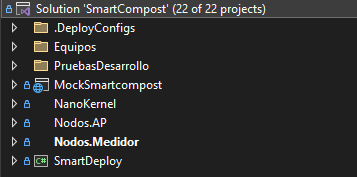
\includegraphics[width=0.8\linewidth]{Figures//Firmware/smartcompost_app.png}
    \caption{Estructura de proyectos del firmware SmartCompost.}
    \label{fig:estructura-codigo-firmware}
\end{figure}

En el Apéndice B se encuentran extractos del código principal de los Nodos Sensor y AP.

%----------------------------------------------------------------------------------------
%	SECCIÓN - PORTAL WEB
%----------------------------------------------------------------------------------------
\section{Portal Web}


%----------------------------------------------------------------------------------------
%	SUBSECCIÓN - ARQUITECTURA DEL SISTEMA
%----------------------------------------------------------------------------------------
\subsection{Arquitectura del sistema}

La arquitectura del sistema está diseñada para ser eficiente y escalable, aprovechando un enfoque basado en microservicios y contenedores. En el núcleo de esta arquitectura se encuentra un \textit{ reverse proxy}, implementado con Nginx, el cual actúa como el punto de entrada para todas las solicitudes, tanto de los usuarios como de nuestra API dedicada a recibir datos de los Nodos Access Point centrales.

Nginx se encarga de redirigir las solicitudes, enviando las peticiones al \textit{backend} o al \textit{frontend} según corresponda. Esta capa de proxy inverso no solo optimiza la distribución del tráfico, sino que también proporciona un nivel adicional de seguridad y flexibilidad, facilitando el manejo del enrutamiento y la gestión de cargas.

En la Figura \ref{fig:arquitecturaweb} se puede observar un diagrama de la arquitectura web general del sistema, demostrando en color rojo el camino que realiza la comunicación desde el Nodo Access Point hacia el Portal web, y por otro lado, en color amarillo el acceso de los usuarios a través de la página hacia el Frontend.

\begin{figure}[H]
    \adjustbox{center=15cm}{
        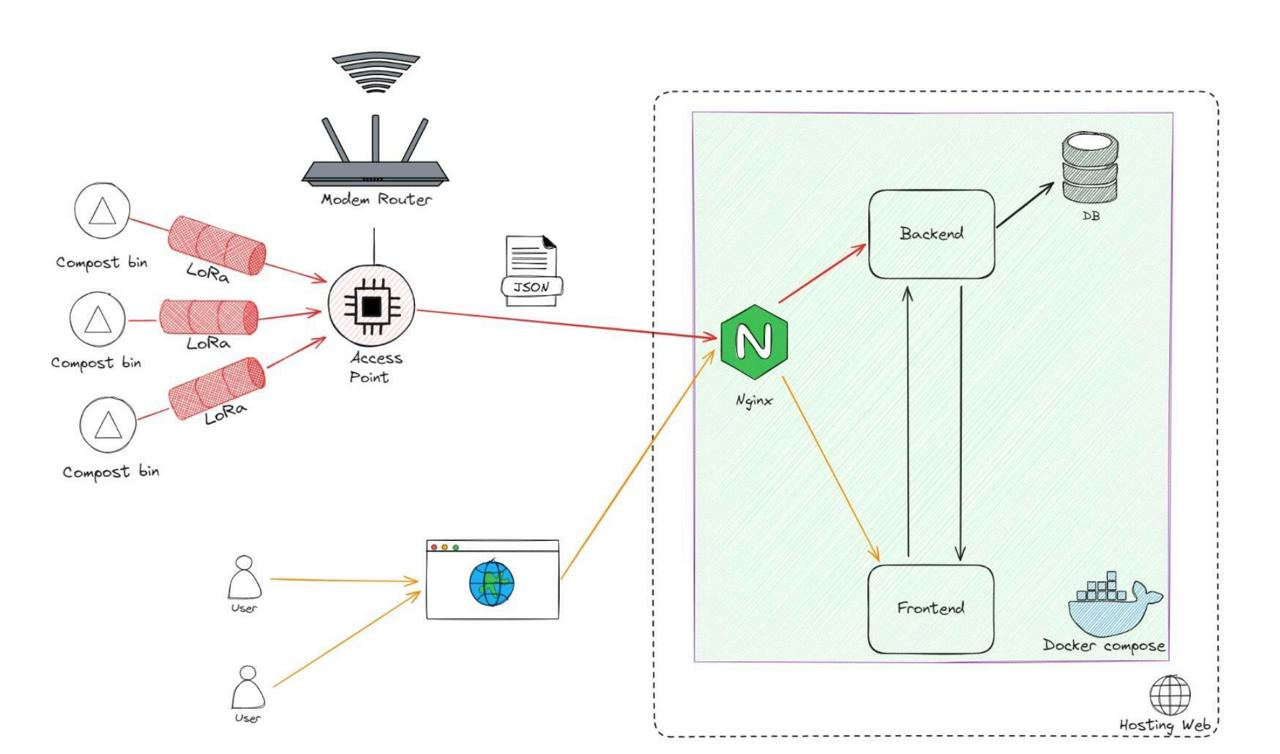
\includegraphics[scale=.4]{./Figures/PortalWeb/Arquitectura web smartcompost.jpeg}
    }
    \caption{Arquitectura web general sobra la comunicación con el Portal web de Smartcompost.}
    \label{fig:arquitecturaweb}
\end{figure}

Para garantizar un entorno de desarrollo y producción consistente y fácil de administrar, se utilizo Docker Compose \citep{DockerCompose}. Esta herramienta permite \textit{containerizar} todos los componentes del sistema, asegurando que cada servicio se ejecute en un entorno controlado y aislado. Esto facilita no solo el despliegue inicial, sino también la reimplementación y el escalado del sistema cuando es necesario. También simplifica la reproducción del entorno en diferentes máquinas, lo que es crucial para pruebas y despliegues en múltiples ambientes.

%----------------------------------------------------------------------------------------
%	SUBSECCIÓN - frontend
%----------------------------------------------------------------------------------------
\subsection{Frontend}

En primera instancia se desarrolló una capa de presentación aplicando la tecnología ReactJS con la finalidad de ser utilizada por los usuarios del sistema y así lograr gestionar sus composteras, los parámetros de sus nodos y administrar el estado general de compostaje. 

La administración de los usuarios estaría orientada a organizaciones que inician su sesión en una capa de logueo como se indica en la Figura \ref{fig:login}. 

\begin{figure}[H]
	\centering
	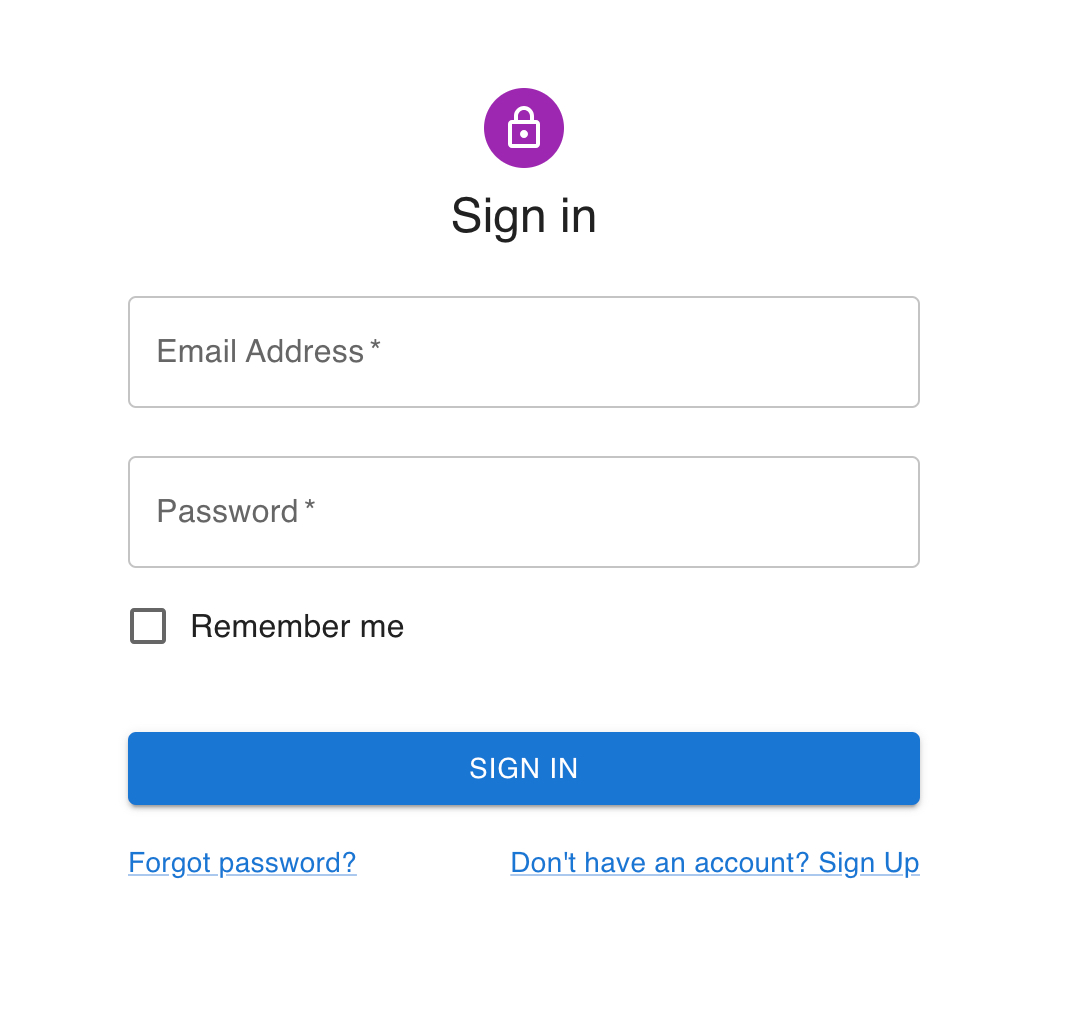
\includegraphics[scale=.2]{./Figures/PortalWeb/Login.jpeg}
	\caption{Pantalla de login.}
	\label{fig:login}
\end{figure}

Dentro de la sesión de cada usuario se puede observar el estado de cada uno de sus Nodos Access Point diferenciando cromáticamente y con un label su nivel de batería, tal como se indica en la Figura \ref{fig:Dash}. 

\begin{figure}[H]
	\centering
	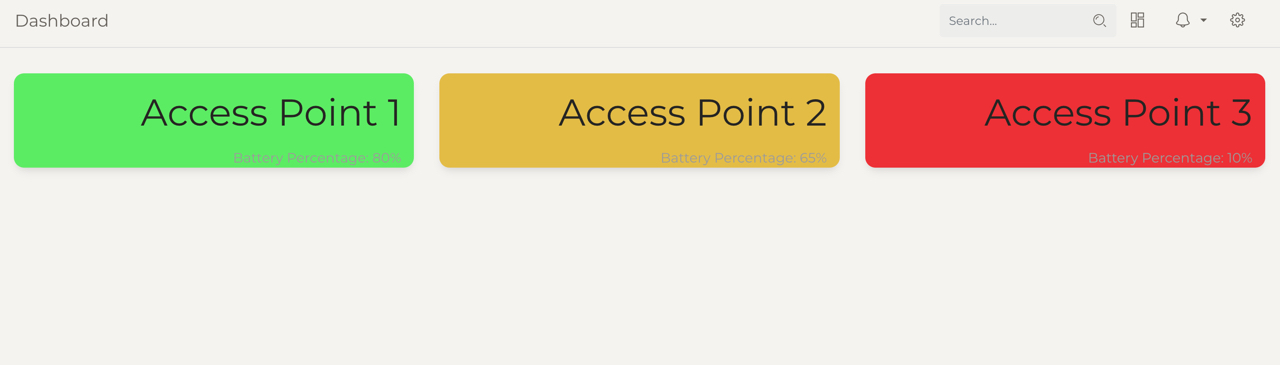
\includegraphics[scale=.3]{./Figures/PortalWeb/Dashboard-composteras.jpeg}
	\caption{Dashboard principal del estado de las composteras.}
	\label{fig:Dash}
\end{figure}

Finalmente, de forma sencilla e intuitiva, al ingresar en cada uno de los Nodos AP se podría demostrar en mayor detalle los parámetros de cada compostera asociada como se observa en la Figura \ref{fig:web-detalles-nodoAP}. 

\begin{figure}[H]
    \centering
    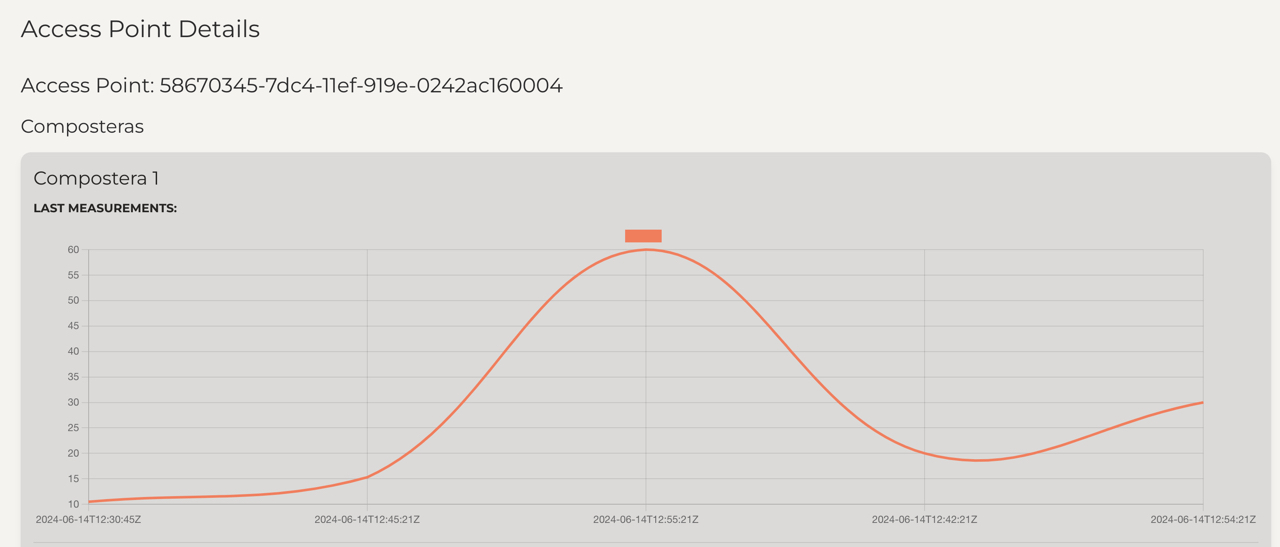
\includegraphics[scale=0.35]{./Figures/PortalWeb/Detalles-compsotera.jpeg}
	\caption{Detalles de los parámetros de cada Nodo Access Point.}
 \label{fig:web-detalles-nodoAP}
\end{figure}

Sin embargo, se tomó la decisión de no dar demasiado énfasis al desarrollo del frontend, optando por dar una orientación administrativa del sistema, es decir, el diseño y desarrollo del frontend se centraron en proporcionar herramientas básicas y funcionales para la gestión de los datos recopilados por los nodos. Es por ello que se incluye una interfaz que permite a los administradores visualizar mediciones clave y monitorear el estado de sus nodos de manera sencilla, priorizando la funcionalidad del sistema y de la lógica del backend por sobre la estética.


\subsubsection{Diseño final del backoffice}

Para garantizar un control adecuado del sistema y obtener visibilidad sobre su rendimiento, se buscó una solución eficiente para observar y monitorear los datos en tiempo real. Durante este proceso, se evaluaron diversas herramientas, como Kibana, que aunque potente, resultaba demasiado demandante en cuanto a recursos. También se consideró Datadog, una opción robusta pero con un costo elevado que no se ajustaba al presupuesto del proyecto.

Finalmente, se optó por integrar Grafana, una herramienta que ofrece un equilibrio ideal entre funcionalidad y eficiencia, permitiendo la visualización de datos tanto desde la base de datos MySQL como desde los logs del backend y del reverse proxy Nginx. A continuación, en la Figura \ref{fig:grafana-dashboard} se presentan ejemplos de los dashboards utilizados para este monitoreo.

\begin{figure}[H]
	\centering
	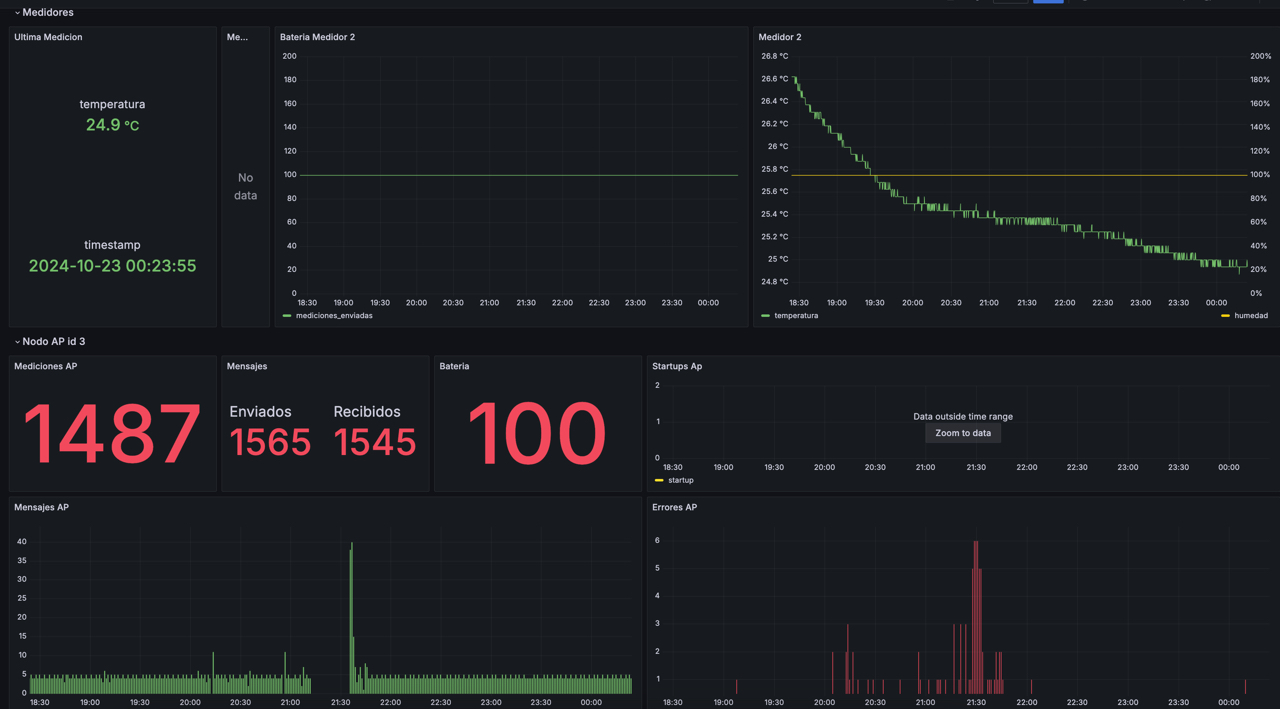
\includegraphics[scale=.3]{./Figures/PortalWeb/Grafana-dashboard.jpeg}
	\caption{Dashboards de Grafana.}
	\label{fig:grafana-dashboard}
\end{figure}

Esta herramienta permite, de un simple vistazo, ver las mediciones, verificar que los datos enviados y recibidos son los esperados y comprobar que nuestro sistema se encuentra activo y en correcto funcionamiento, dando simplicidad tanto al desarrollo del mismo como a la posterior implementación. 

Además, esto brinda trazabilidad para poder depurar el sistema y/o capturar el momento exacto donde pudiera haberse perpetuado una falla. 





%----------------------------------------------------------------------------------------
%	SUBSECCIÓN - backend
%----------------------------------------------------------------------------------------
\subsection{Backend}
\subsubsection{Selección de lenguaje y tecnologías}

Para el desarrollo del backend de SmartCompost se eligió Golang debido a sus características que estan alineadas con las necesidades específicas del proyecto. La claridad y simplicidad de su sintaxis no solo agilizan el desarrollo, sino que también permite a los miembros del equipo que no están familiarizados con el desarrollo backend comprender y colaborar más fácilmente en el código. 

Una de las ventajas más relevantes para SmartCompost es que Golang, al ser un lenguaje compilado, permite dividir las tareas del backend en binarios independientes. De esta manera se puede pensar en escalar el sistema, pudiendo repartir las responsabilidades de la API usada por los administradores para la carga de nuevos usuarios/organizaciones, con las asociadas al manejo de datos y respuesta hacia el frontend. 

Por último, el uso de la biblioteca estándar de Golang \cite{GoStdlibTesting} y sus herramientas integradas, como go fmt para formatear código, go test para pruebas unitarias y go mod para la gestión de dependencias, simplificaron el desarrollo iterativo. Estas herramientas permiten a los desarrolladores enfocarse en implementar las funcionalidades específicas de SmartCompost, reduciendo la necesidad de soluciones externas y optimizando los tiempos de desarrollo y pruebas.


\subsubsection{Arquitectura utilizada}
Para la estructura del backend, se optó por una arquitectura hexagonal \citep{ArquitecturaHexagonal:15} combinada con principios de \textit{Domain-Driven Design (DDD)}\cite{Evans2003}. Este enfoque permitió desarrollar un sistema modular y flexible como se puede observar en la Figura \ref{fig:arquitecturahexagonal}\citep{ArquitecturaHexagonal:15}, donde las diferentes capas de la aplicación están claramente separadas, promoviendo la independencia de las reglas de negocio con respecto a los detalles de infraestructura.


\begin{figure}[H]
	\centering
	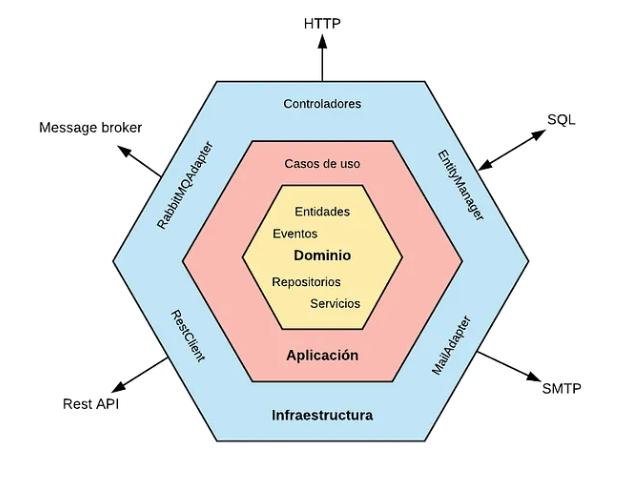
\includegraphics[scale=.5]{./Figures/PortalWeb/Arquitectura-Hexagonal.jpeg}
	\caption{Arquitectura hexagonal.}
	\label{fig:arquitecturahexagonal}
\end{figure}

En conjunto, la combinación de la arquitectura hexagonal y DDD  brinda una base sólida para desarrollar un backend que no solo es robusto y escalable, sino también fácil de mantener y extender a medida que evolucionan las necesidades del sistema. 

Un ejemplo concreto de las ventajas de la arquitectura hexagonal se evidenció cuando se decidió cambiar la base de datos de Postgres a MySQL. Este cambio fue impulsado por la necesidad de aprovechar ciertas características y optimizaciones de MySQL que se adaptaban mejor a las necesidades de rendimiento y escalabilidad.

Gracias a la arquitectura hexagonal, este proceso fue sencillo. Como la lógica de negocio estaba desacoplada de los detalles específicos de la base de datos, solo se necesitó ajustar los adaptadores que conectaban el núcleo de la aplicación con el sistema de persistencia. Esto significó que el resto de la aplicación, incluyendo las reglas de negocio y los servicios de dominio permanecieran inalterados, tal como se observa en la Figura \ref{fig:modifAdapters}. 

\begin{figure}[H]
	\centering
	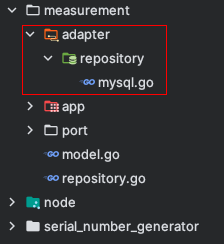
\includegraphics[scale=.7]{./Figures/PortalWeb/Ej_cambio-adapters.png}
	\caption{Arquitectura hexagonal - Modificación de adapters.}
	\label{fig:modifAdapters}
\end{figure}

\subsubsection{Testing}
Para el testing del proyecto, se adoptó un enfoque exhaustivo que incluyó varias técnicas para asegurar la calidad y el rendimiento del sistema. En primer lugar, se implementaron \textit{unit tests} e \textit{integration tests} empleando la biblioteca estándar de Go \cite{GoStdlibTesting}. Estos tests permitieron verificar el correcto funcionamiento de cada componente de manera aislada y en conjunto, alcanzando un nivel de cobertura de código superior al 80\% para el backend. Este alto porcentaje de cobertura confirmó la fiabilidad y estabilidad del código.

Además, se desarrolló una aplicación específica llamada \textit{simulator} para realizar pruebas de carga. Esta herramienta se diseño para enviar datos de manera aleatoria y simular condiciones de uso intensivo. Los resultados de las pruebas de carga demostraron que el sistema era capaz de soportar hasta 10 mediciones por segundo, con un percentil 99 (p99) que indicaba que el 99\% de las mediciones se procesaban dentro de un tiempo de respuesta específico. Estos resultados confirmaron que el proyecto está preparado para manejar las cargas esperadas en un entorno de producción, garantizando un rendimiento robusto y consistente.




%----------------------------------------------------------------------------------------
%	SUBSECCIÓN - BASE DE DATOS
%----------------------------------------------------------------------------------------
\subsection{Base de Datos}

Para el almacenamiento de datos en el proyecto, se eligió MySQL, una base de datos relacional ampliamente reconocida en la industria del software. Las bases de datos relacionales, como MySQL, ofrecen ventajas significativas, como la integridad de datos mediante la definición de restricciones como claves primarias y foráneas, la capacidad para realizar consultas complejas a través de SQL, y la normalización que reduce la redundancia de datos. Además, soportan transacciones ACID, lo que asegura operaciones confiables y consistentes.

En el modelo de datos del proyecto que se muestra en la Figura \ref{fig:db_diagram}, se definieron varias tablas clave: \textit{nodes}, \textit{measurements}, \textit{users} y \textit{organizations}. La tabla nodes gestiona la información de los nodos del sistema, incluyendo un identificador único, número de serie, descripción, modelo, y referencias a la organización a la que pertenecen. La tabla measurements almacena las mediciones asociadas a cada nodo, registrando el valor, el tipo de medición y la fecha y hora de la toma de datos. Por otro lado, la tabla users contiene la información de los usuarios del sistema, incluyendo nombre de usuario, contraseña (hashificada para seguridad), el identificador de la organización a la que pertenecen, y su rol. Finalmente, la tabla organizations define las organizaciones que gestionan los nodos y usuarios, proporcionando una estructura organizativa clara.

\begin{figure}[H]
	\centering
	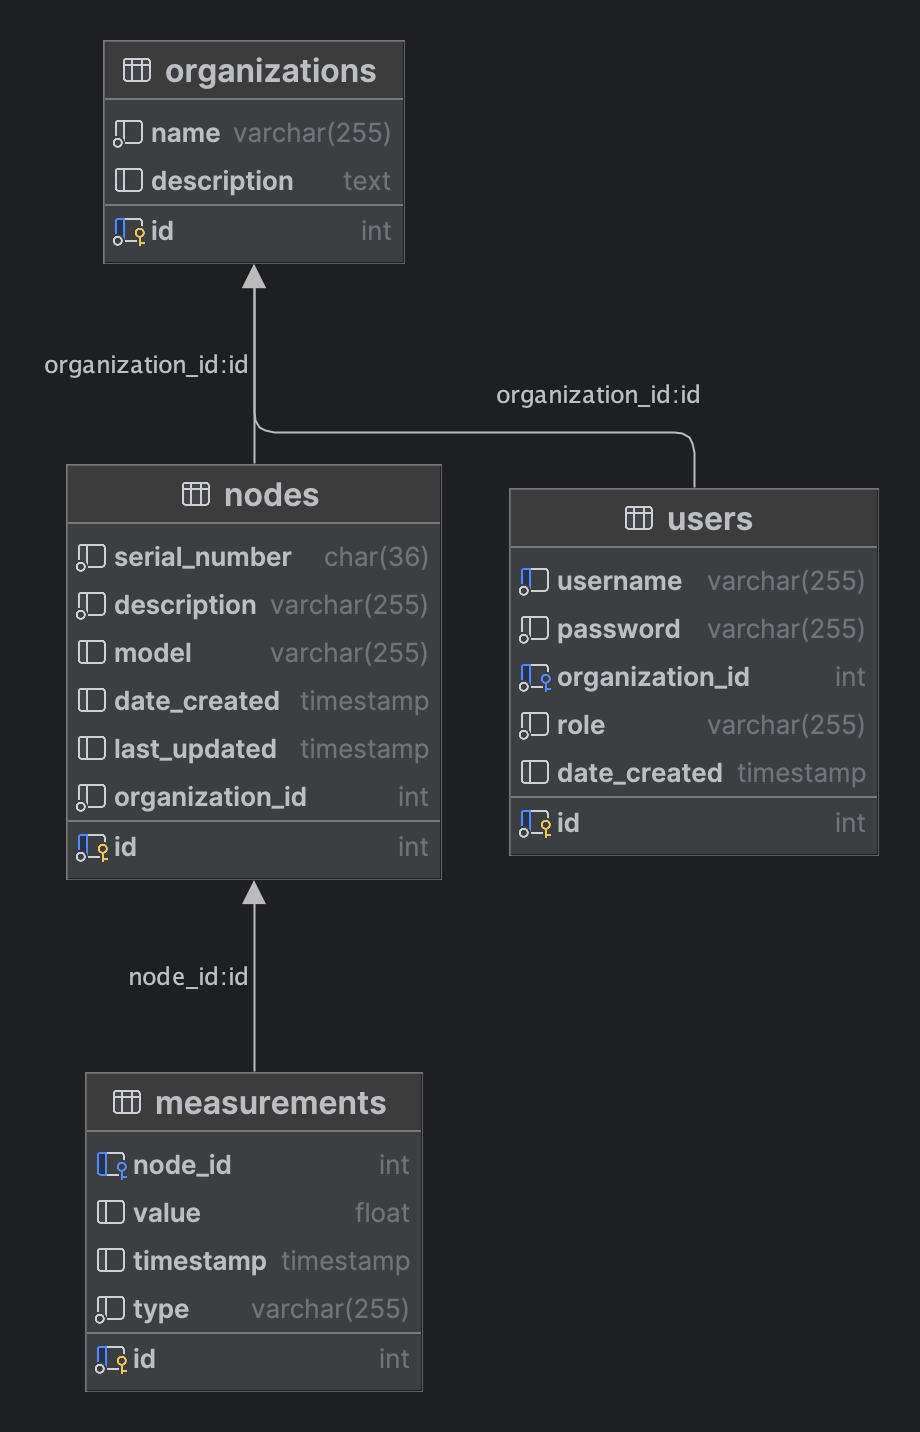
\includegraphics[scale=.2]{./Figures/PortalWeb/smartcompost_db.png}
	\caption{Diagrama de Base de Datos.}
	\label{fig:db_diagram}
\end{figure}

Durante el desarrollo, se realizó un cambio de PostgreSQL a MySQL basándose en varios factores que resultaban favorables para este proyecto. El equipo de desarrollo ya contaba con una sólida experiencia en esta tecnología, lo que facilitó un desarrollo más ágil y una resolución de problemas más efectiva. MySQL también ofrece un rendimiento robusto y una buena capacidad de manejo de grandes volúmenes de datos, así como un soporte extenso de la comunidad y documentación que simplifica la integración con otras tecnologías. Además, en algunos casos, los costos asociados con PostgreSQL pueden ser mayores, mientras que MySQL, siendo una opción de código abierto, puede resultar más económico.

%----------------------------------------------------------------------------------------
%	SUBSECCIÓN - CONTAINERIZACION
%----------------------------------------------------------------------------------------
\subsection{Containerización}

La containerización a través de \textit{Docker Compose} es un instrumento clave para garantizar la portabilidad y facilidad de despliegue. Al mantener todos los servicios en contenedores, se logra aislar cada componente del sistema, como son el servidor Nginx, el backend en Go, la base de datos MySQL, el frontend en React y el backoffice Grafana como se puede observar en el apéndice \ref{AppendixA}. Esta modularidad facilita la administración, ya que cada servicio tiene su propio contenedor y puede ser escalado o modificado independientemente de los demás. Además, de esta manera la containerización asegura que los entornos de desarrollo y producción sean idénticos, eliminando problemas derivados a raiz de diferencias entre ellos. 
En la Figura \ref{fig:docker-compose} se presenta el modelo final de los containers utilizados para el desarrollo global del Portal Web.

\begin{figure}[H]
	\centering
	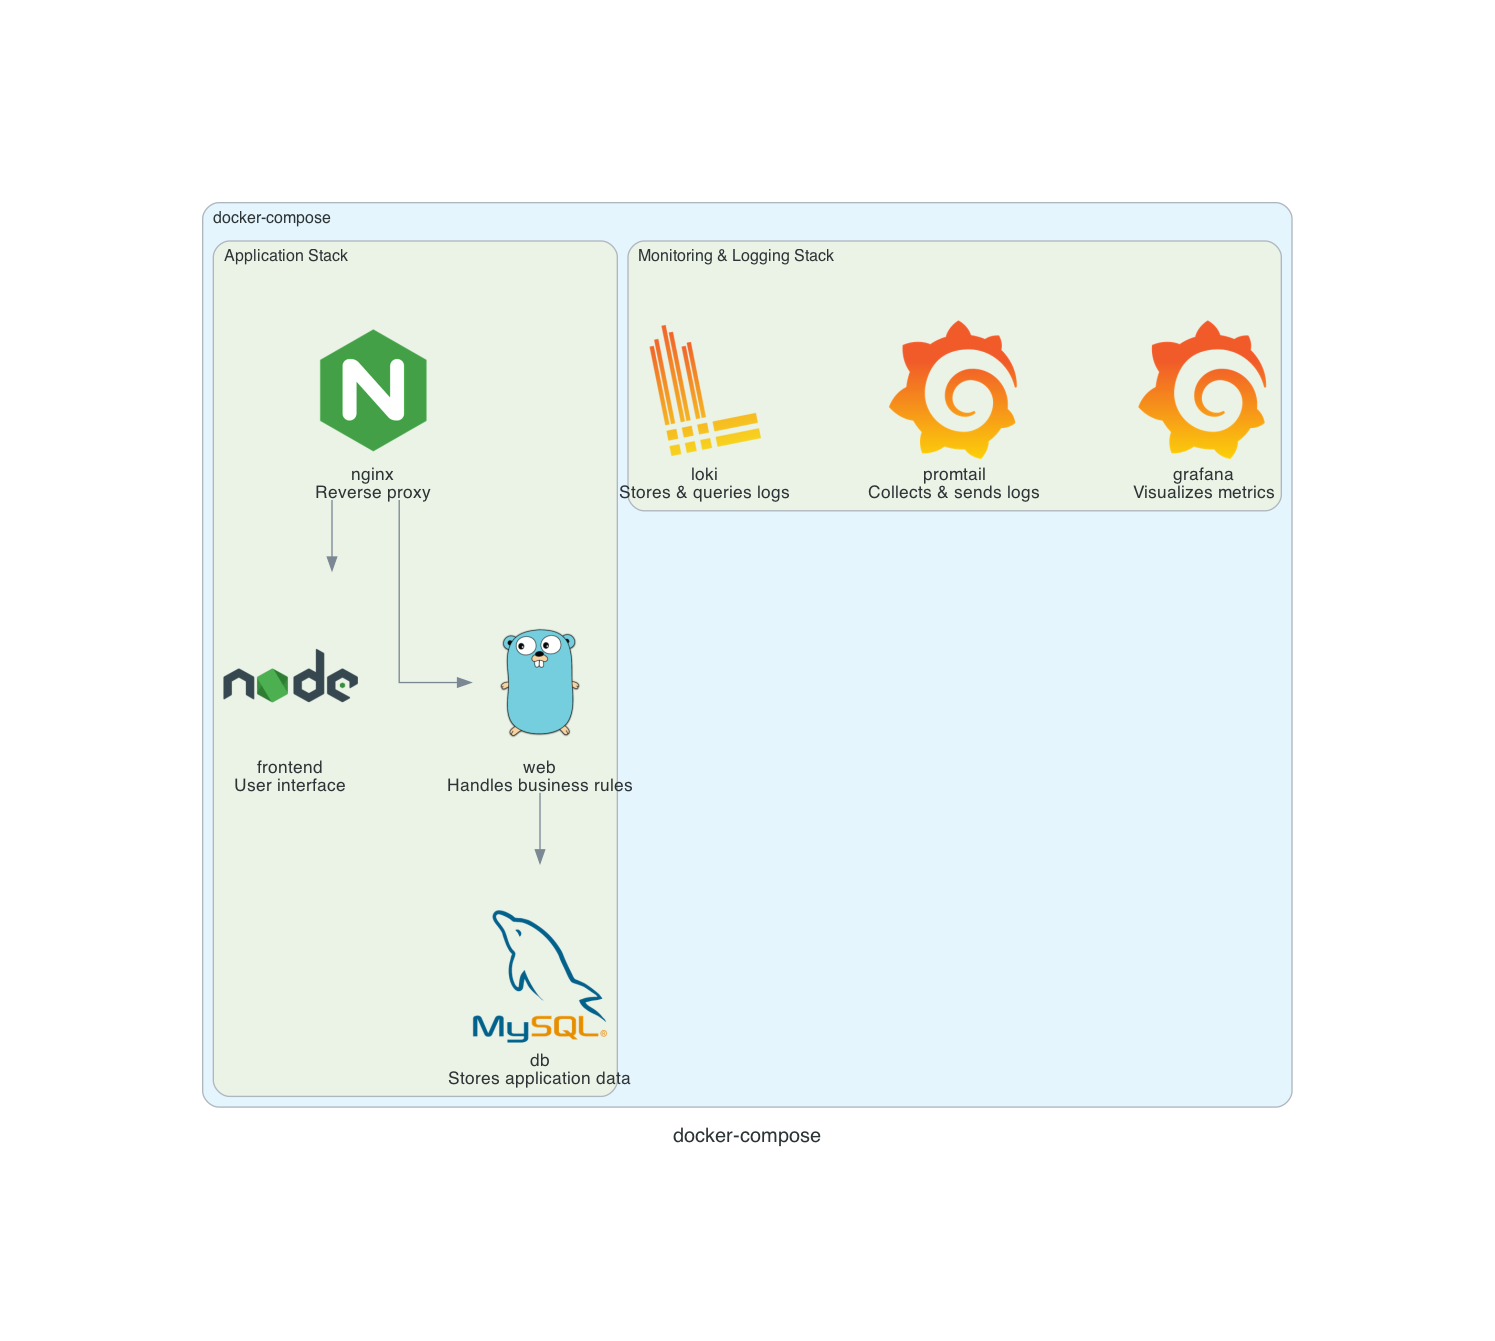
\includegraphics[scale=.29]{./Figures/PortalWeb/docker-compose.png}
	\caption{Orquestación de containers.}
	\label{fig:docker-compose}
\end{figure}

El uso de redes personalizadas dentro de la separación de containers permite segmentar el tráfico entre los servicios y así evitar que componentes no relacionados se comuniquen directamente. Esto mejora la seguridad del sistema, al mantener una arquitectura en la que sólo los servicios necesarios pueden interactuar entre sí. Por ejemplo, la red \textit{logging} conecta únicamente a Promtail, Loki y Grafana, encargados de la recolección y visualización de logs, sin permitir acceso al resto de los servicios.

En cuanto a los volúmenes, estos proporcionan persistencia de datos, algo crítico para servicios como la base de datos MySQL. Se definieron volúmenes para asegurar que los datos no se pierdan tras un reinicio o actualización de los contenedores. Además, los volúmenes son fundamentales para centralizar los logs generados por servicios como Nginx, el backend, y MySQL, lo que facilitó el monitoreo y diagnóstico de problemas al almacenar los archivos de logs en ubicaciones accesibles de manera permanente.

El control del orden de despliegue con la opción \textit{depends\_on} también resultó esencial. Al asegurarse de que la base de datos esté operativa antes de que el backend se inicie, o que el frontend no comience a recibir tráfico antes de que Nginx esté listo, se logra evitar errores de inicialización. Esto garantiza que todo el sistema se levante de manera ordenada y funcional desde el primer momento, sin generar fallos por servicios no disponibles.

%----------------------------------------------------------------------------------------
%	SUBSECCIÓN - HOSTING
%----------------------------------------------------------------------------------------
\subsection{Hosting}

Para el despliegue del proyecto, se evaluaron varias opciones de \textit{hosting} y, finalmente, se optaron por los servicios de Donweb \citep{DonwebWebsite}, específicamente por su oferta de \textit{cloud} e infraestructura como servicio (IaaS por sus siglas en inglés). Esta decisión se tomó debido a la flexibilidad que ofrece su plataforma, permitiendo una escalabilidad sencilla y una gestión eficiente de los recursos. Además, Donweb proporcionó el entorno adecuado para el manejo de contenedores Docker, facilitando el proceso de implementación y mantenimiento del sistema con una fácil comunicación local a través de ssh.

Dentro de las características específicas que nos ofrece Donweb como plataforma de hosting, se encuentran la forma simplificada de utilizar herramientas de seguridad como un Firewall o realizar copias de seguridad, tanto como una visión integral de las métricas asociadas a las estadísticas de uso, como se puede observar en la Figura \ref{fig:metricas-donweb}.

%%%%%%%%
\begin{figure}[H]
    \centering
    % Primera fila
    \begin{subfigure}[b]{0.45\textwidth}
        \centering
        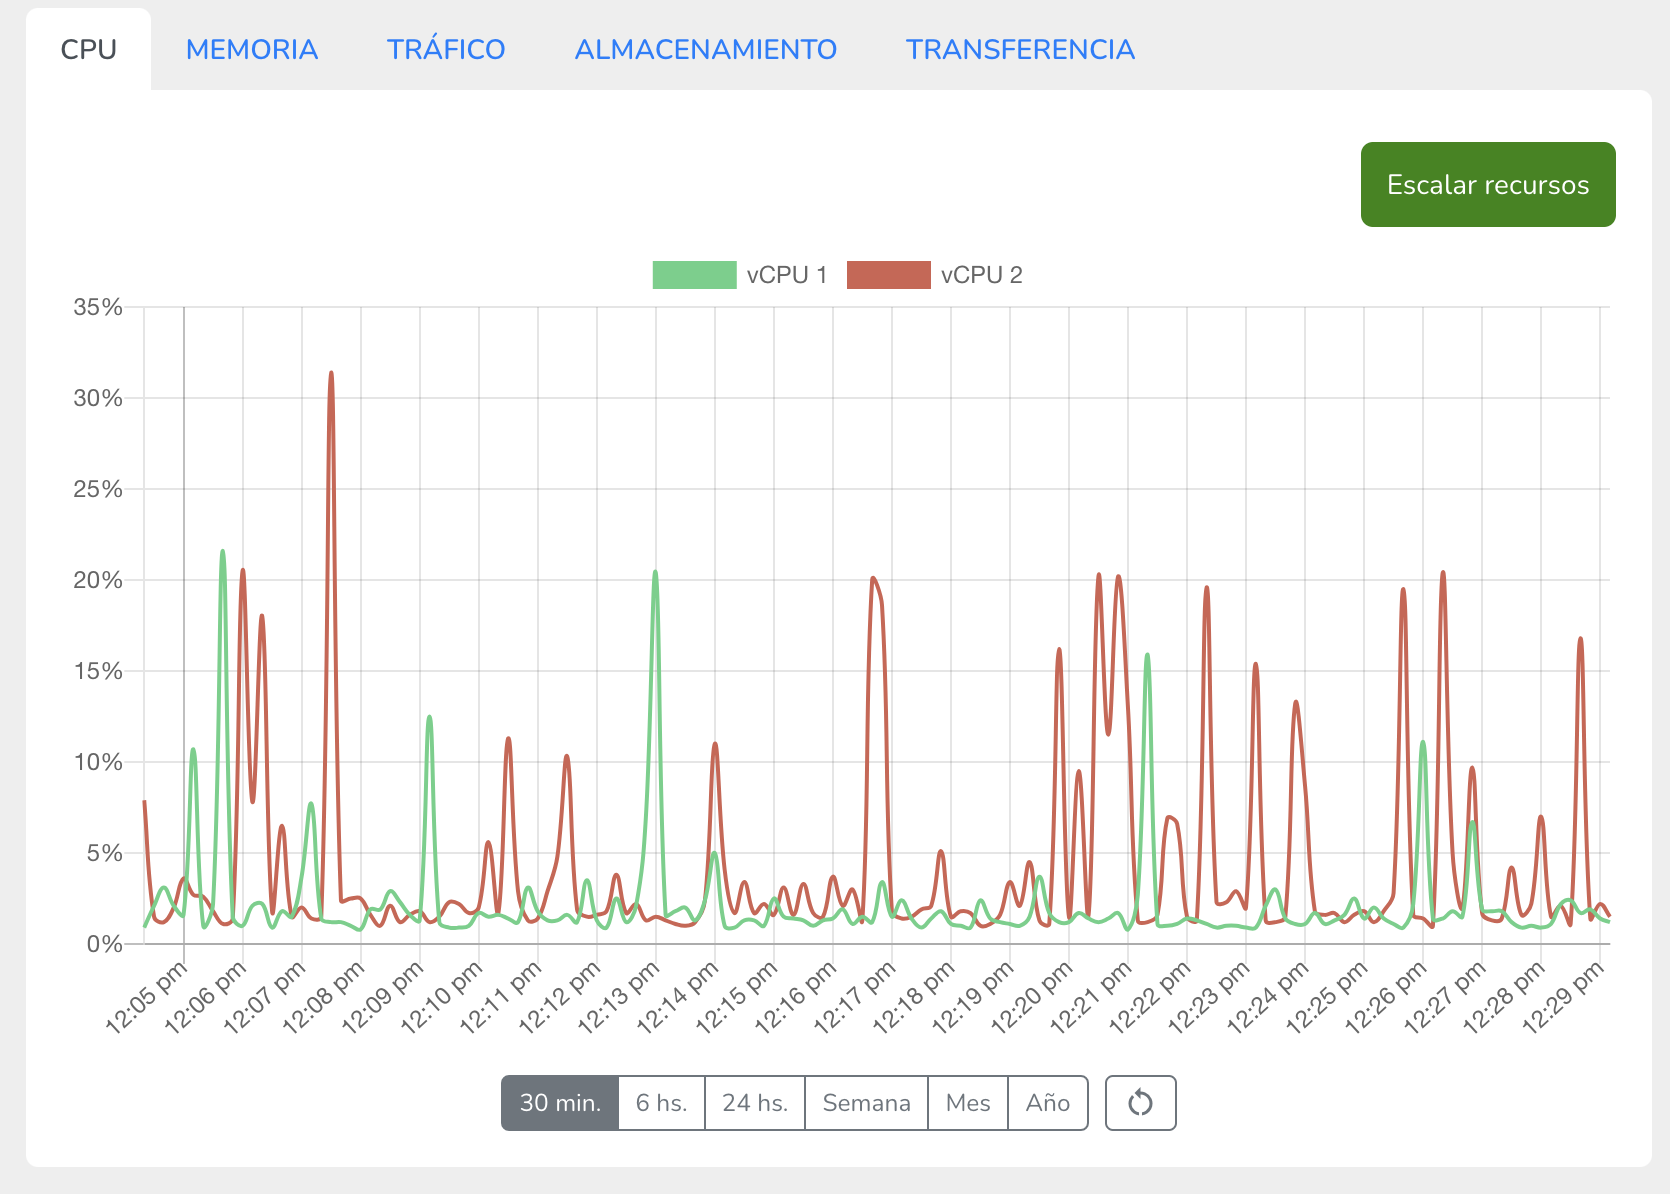
\includegraphics[width=\textwidth]{Figures/PortalWeb/CPU-Donweb.png}
        \caption{Uso de CPU en Donweb.}
        \label{fig:cpu-donweb}
    \end{subfigure}
    \hfill
    \begin{subfigure}[b]{0.45\textwidth}
        \centering
        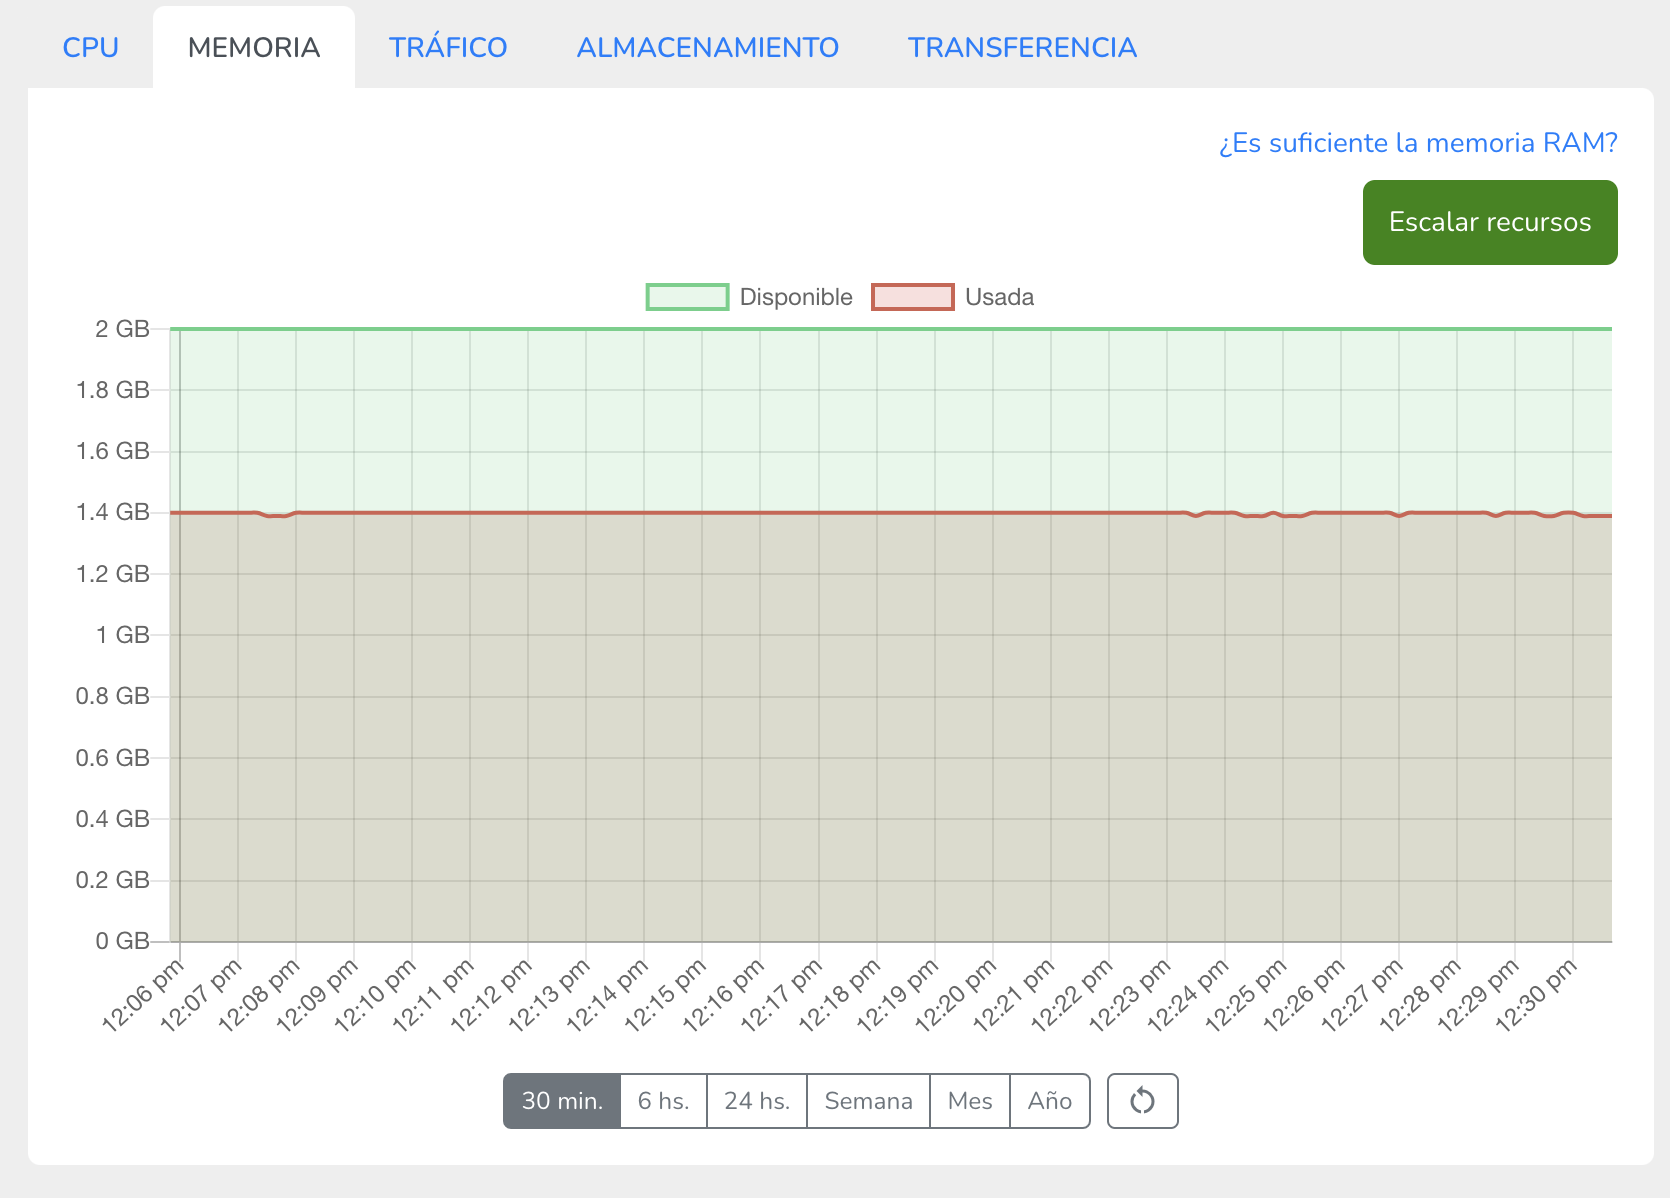
\includegraphics[width=\textwidth]{Figures/PortalWeb/Memoria-Donweb.png}
        \caption{Uso de Memoria en Donweb.}
        \label{fig:memoria-donweb}
    \end{subfigure}
    
    % Segunda fila
    \begin{subfigure}[b]{0.45\textwidth}
        \centering
        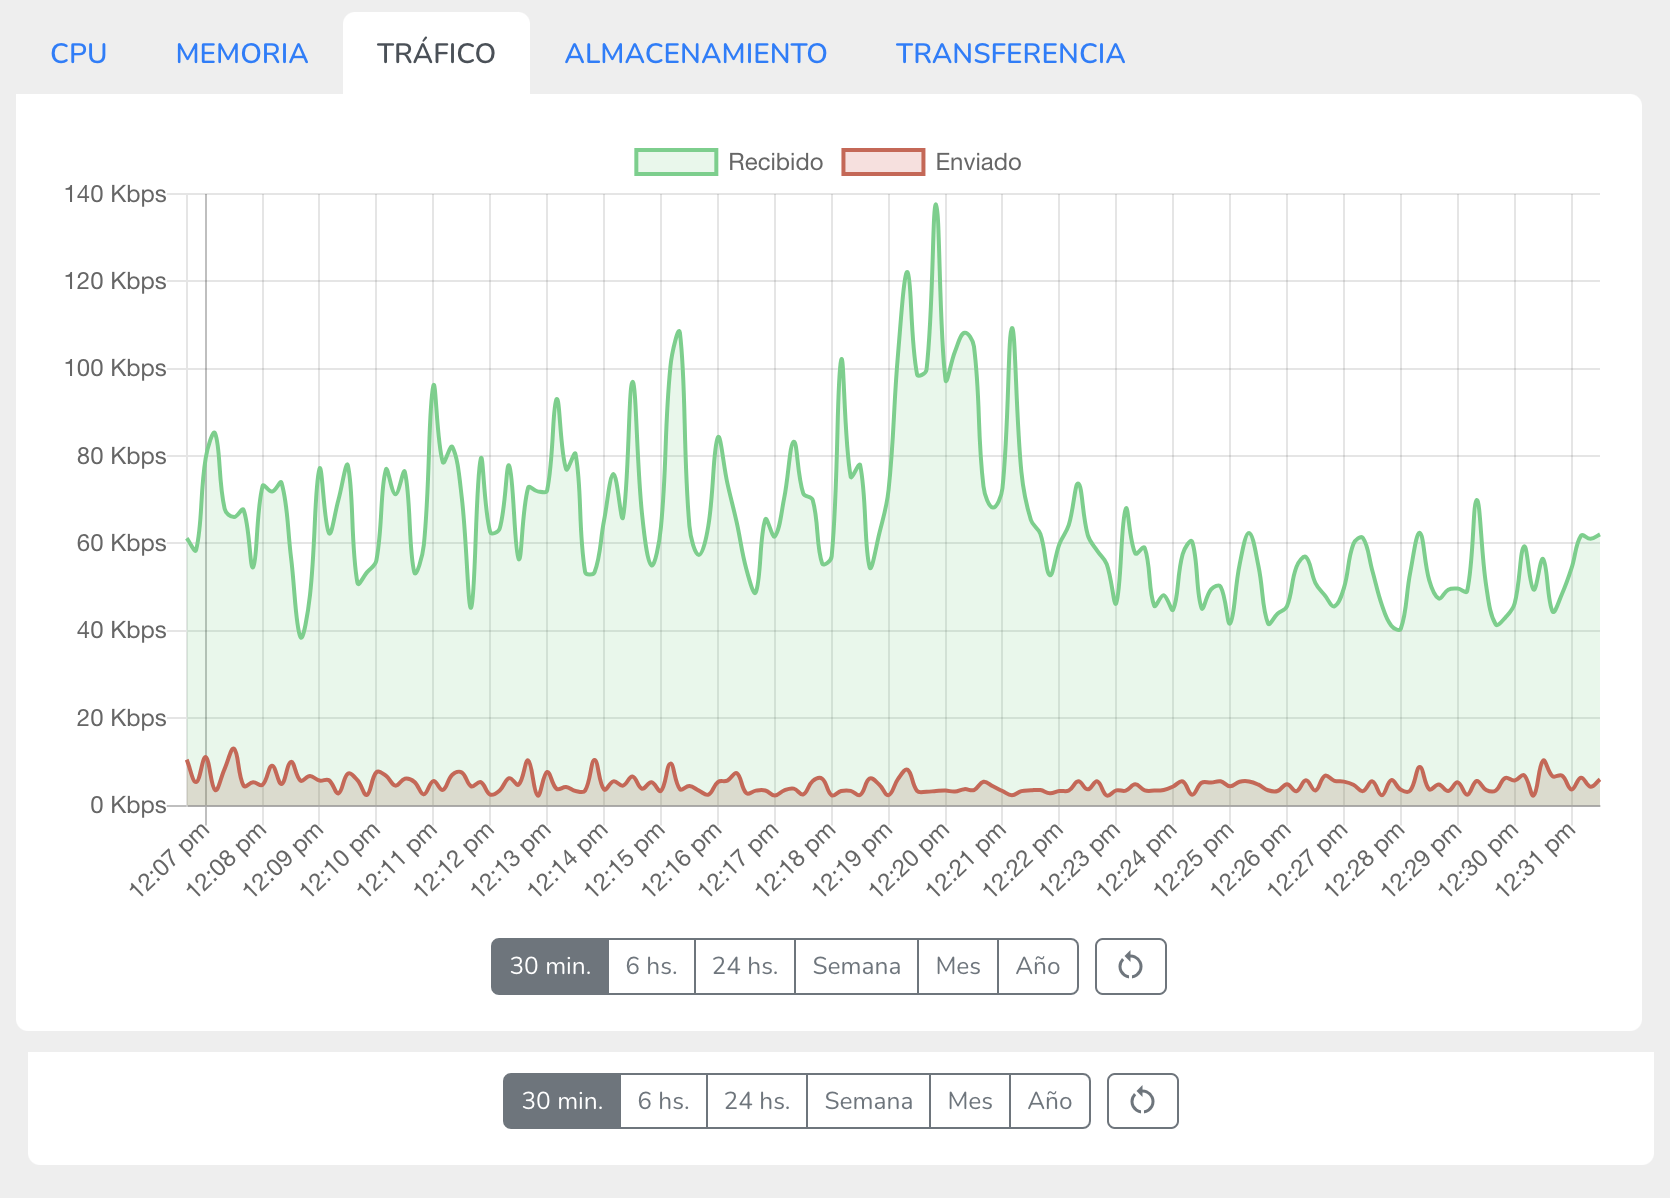
\includegraphics[width=\textwidth]{Figures/PortalWeb/Trafico-Donweb.png}
        \caption{Tráfico de Red en Donweb.}
        \label{fig:trafico-donweb}
    \end{subfigure}
    \hfill
    \begin{subfigure}[b]{0.45\textwidth}
        \centering
        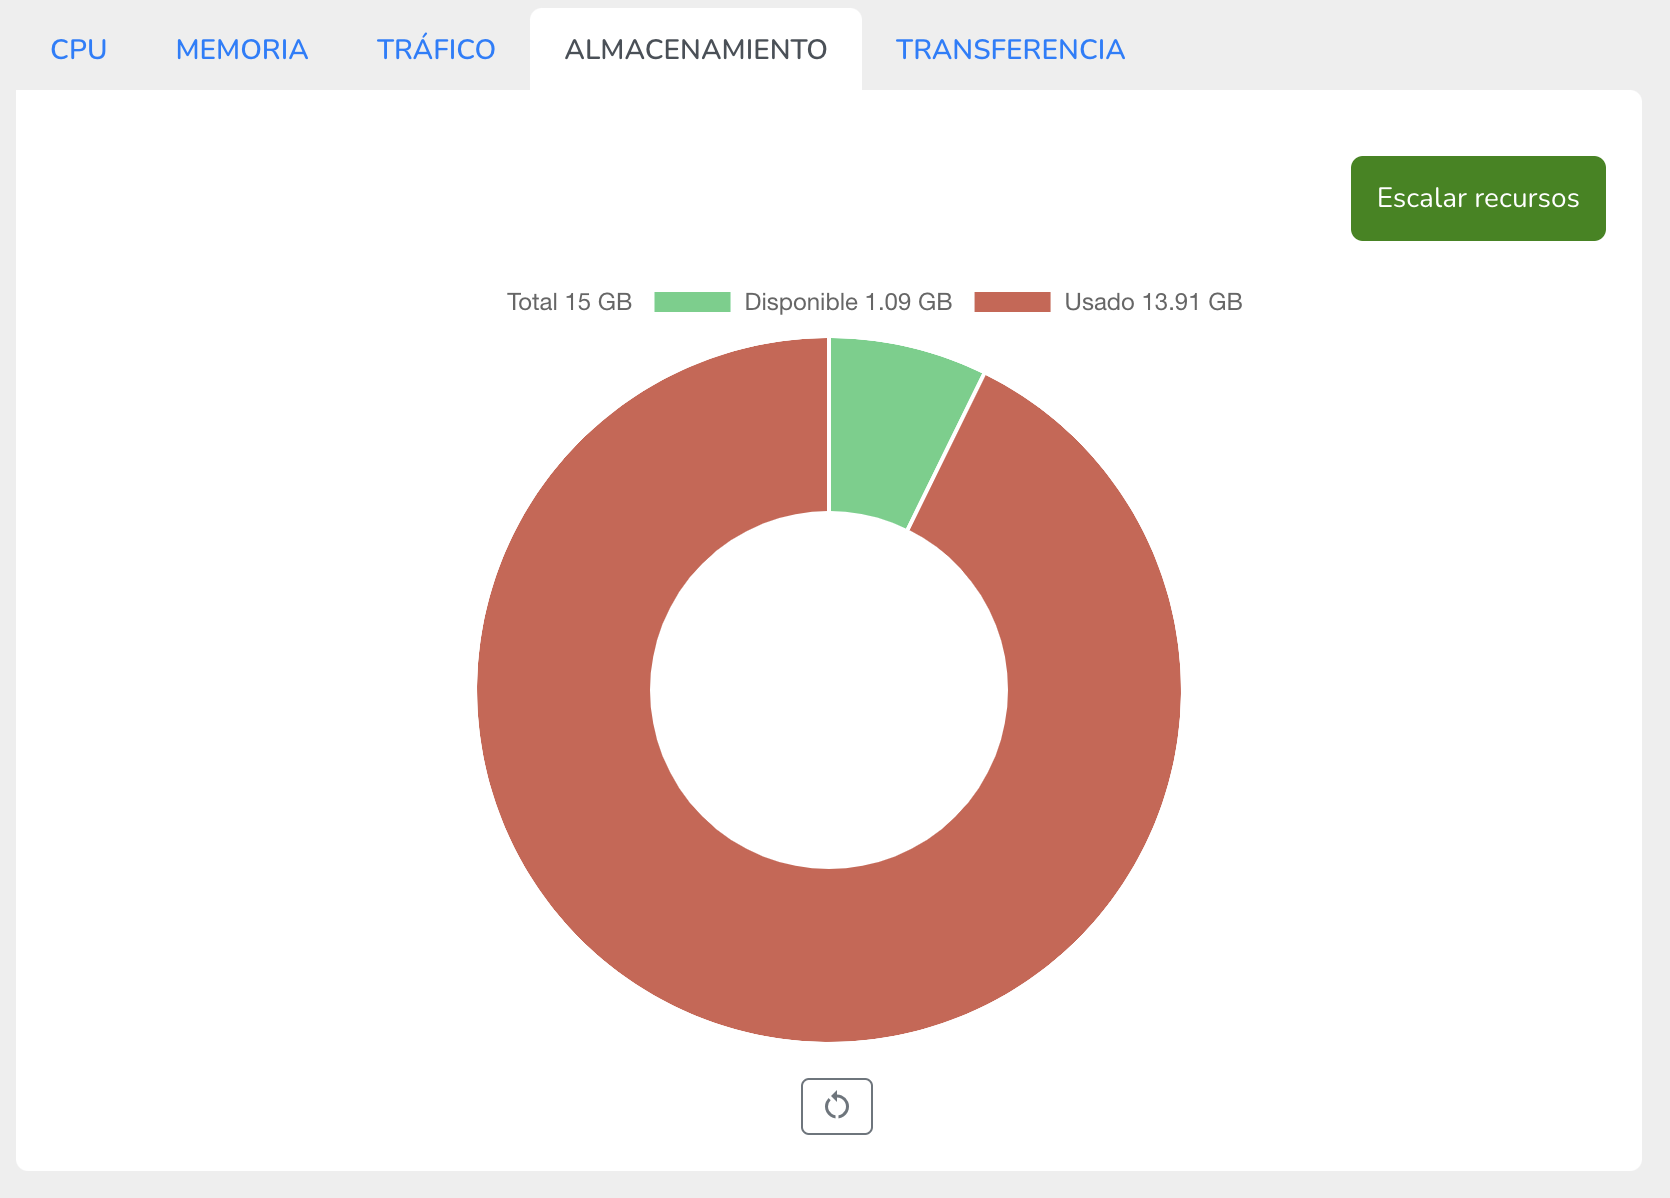
\includegraphics[width=\textwidth]{Figures/PortalWeb/Almacenamiento-Donweb.png}
        \caption{Uso de Almacenamiento en Donweb.}
        \label{fig:almacenamiento-donweb}
    \end{subfigure}
    
    \caption{Métricas del hosting en Donweb.}
    \label{fig:metricas-donweb}
\end{figure}


%%%%%%%%

Otra opción considerada fue utilizar los servicios de AWS \citep{AWSWebsite} debido a su gran capacidad de escalabilidad y la variedad de servicios que ofrece. Sin embargo, se decidió no optar por AWS principalmente debido a la complejidad adicional que implica su configuración y gestión, así como a los costos que, en algunos casos, pueden ser superiores a los de otros proveedores como Donweb. Además, el equipo ya contaba con experiencia previa utilizando Donweb, lo que facilitó la integración y el despliegue del proyecto sin necesidad de invertir tiempo adicional en aprender nuevas herramientas o adaptarse a una infraestructura más compleja.

%----------------------------------------------------------------------------------------
%	SUBSECCIÓN - MANEJO DE LOGS Y DASHBOARDS
%----------------------------------------------------------------------------------------






%----------------------------------------------------------------------------------------
%	AYUDA SOBRE COMO ESCRIBIR CÓDIGO
%----------------------------------------------------------------------------------------
% \definecolor{mygreen}{rgb}{0,0.6,0}
% \definecolor{mygray}{rgb}{0.5,0.5,0.5}
% \definecolor{mymauve}{rgb}{0.58,0,0.82}

%%%%%%%%%%%%%%%%%%%%%%%%%%%%%%%%%%%%%%%%%%%%%%%%%%%%%%%%%%%%%%%%%%%%%%%%%%%%%
% parámetros para configurar el formato del código en los entornos lstlisting
%%%%%%%%%%%%%%%%%%%%%%%%%%%%%%%%%%%%%%%%%%%%%%%%%%%%%%%%%%%%%%%%%%%%%%%%%%%%%
% \lstset{ %
  % backgroundcolor=\color{white},   % choose the background color; you must add \usepackage{color} or \usepackage{xcolor}
  % basicstyle=\footnotesize,        % the size of the fonts that are used for the code
  % breakatwhitespace=false,         % sets if automatic breaks should only happen at whitespace
  % breaklines=true,                 % sets automatic line breaking
  % captionpos=b,                    % sets the caption-position to bottom
  % commentstyle=\color{mygreen},    % comment style
  % deletekeywords={...},            % if you want to delete keywords from the given language
  %escapeinside={\%*}{*)},          % if you want to add LaTeX within your code
  %extendedchars=true,              % lets you use non-ASCII characters; for 8-bits encodings only, does not work with UTF-8
  %frame=single,	                % adds a frame around the code
  % keepspaces=true,                 % keeps spaces in text, useful for keeping indentation of code (possibly needs columns=flexible)
  % keywordstyle=\color{blue},       % keyword style
  % language=[ANSI]C,                % the language of the code
  %otherkeywords={*,...},           % if you want to add more keywords to the set
  % numbers=left,                    % where to put the line-numbers; possible values are (none, left, right)
  % numbersep=5pt,                   % how far the line-numbers are from the code
  % numberstyle=\tiny\color{mygray}, % the style that is used for the line-numbers
  % rulecolor=\color{black},         % if not set, the frame-color may be changed on line-breaks within not-black text (e.g. comments (green here))
  % showspaces=false,                % show spaces everywhere adding particular underscores; it overrides 'showstringspaces'
  % showstringspaces=false,          % underline spaces within strings only
  % showtabs=false,                  % show tabs within strings adding particular underscores
  % stepnumber=1,                    % the step between two line-numbers. If it's 1, each line will be numbered
  % stringstyle=\color{mymauve},     % string literal style
  % tabsize=2,	                   % sets default tabsize to 2 spaces
  % title=\lstname,                  % show the filename of files included with \lstinputlisting; also try caption instead of title
  % morecomment=[s]{/*}{*/}
% }


%----------------------------------------------------------------------------------------
%	SECTION 1
%----------------------------------------------------------------------------------------
% \section{Análisis del software}
 
% La idea de esta sección es resaltar los problemas encontrados, los criterios utilizados y la justificación de las decisiones que se hayan tomado.

% Se puede agregar código o pseudocódigo dentro de un entorno lstlisting con el siguiente código:

% \begin{verbatim}
% \begin{lstlisting}[caption= "un epígrafe descriptivo"]
	% las líneas de código irían aquí...
% \end{lstlisting}
% \end{verbatim}

% A modo de ejemplo:

% \begin{lstlisting}[label=cod:vControl,caption=Pseudocódigo del lazo principal de control.]  % Start your code-block

% #define MAX_SENSOR_NUMBER 3
% #define MAX_ALARM_NUMBER  6
% #define MAX_ACTUATOR_NUMBER 6

% uint32_t sensorValue[MAX_SENSOR_NUMBER];		
% FunctionalState alarmControl[MAX_ALARM_NUMBER];	//ENABLE or DISABLE
% state_t alarmState[MAX_ALARM_NUMBER];						//ON or OFF
% state_t actuatorState[MAX_ACTUATOR_NUMBER];			//ON or OFF

% void vControl() {

	% initGlobalVariables();
	
	% period = 500 ms;
		
	% while(1) {

		% ticks = xTaskGetTickCount();
		
		% updateSensors();
		
		% updateAlarms();
		
		% controlActuators();
		
		% vTaskDelayUntil(&ticks, period);
	% }
% }
% \end{lstlisting}


% lazyLizardTracer
